\documentclass[10pt]{report}

\usepackage{lukasbuehler_style}

\usepackage{booktabs}
\usepackage{enumitem}
\usepackage{fancyhdr}
\usepackage[a4paper]{geometry}
\usepackage{listings}
\usepackage{placeins}
\usepackage{siunitx}
\usepackage[dvipsnames,svgnames]{xcolor}

\usepackage{tikz}
\usetikzlibrary{shapes,arrows,snakes,matrix,arrows.meta,backgrounds,decorations.pathreplacing,mindmap,trees,intersections}%fit

\usepackage[lowercase]{theoremref}
%\usepackage{tikz-uml}
\usepackage{graphicx}
\usepackage{caption}
\usepackage{subcaption}
\usepackage{verbatim}
\usepackage{verbatimbox}
\usepackage{colortbl}
\usepackage[hidelinks]{hyperref}
\usepackage{pdfpages}
\usepackage{physics}
\usepackage[titletoc,title]{appendix}
\usepackage{booktabs}
\usepackage{cleveref}
\usepackage{float}
\newfloat{Code}{h}{myc}

% New
%\usepackage{datetime}
\usepackage{pgf-umlcd}
\usepackage{pgf-umlsd}
%\usepackage{pgfgantt}
\usepackage{dirtree}
\usepackage{pgfplots}
\usepackage{minted}
\usepackage{algorithm2e}
%\usepackage[toc,page]{appendix}


\captionsetup[subfigure]{subrefformat=simple,labelformat=simple}
\renewcommand\thesubfigure{(\alph{subfigure})}

%\urlstyle{same} % 09.09.2015, http://latex-community.org/forum/viewtopic.php?f=50&t=4191
\bibliographystyle{IEEEtran}

\include{math}
\include{sectioning}
\include{myenvironment}

\newtheorem{theorem}{Theorem} %13.05.2015, https://www.sharelatex.com/learn/Theorems_and_proofs#Proofs
\newtheorem{definition}{Definition}

%\newcommand{\ref}[1] {Fig.\ \ref{#1}}
\newcommand{\lstref}[1] {Lst.\ \ref{#1}}
\newcommand{\tabref}[1] {Tab.\ \ref{#1}}
\newcommand{\secref}[1] {Sec.\ \ref{#1}}
\newcommand{\outref}[1] {Output \ref{#1}}
\newcommand{\enumref}[1] {Appendix \ref{#1}}
\newtheorem{mydef}{Definition}
% \newcommand{\eqsref}[1] {Eq.\ \ref{#1}}

\lstdefinestyle{MyLstDesign}{
    basicstyle=\scriptsize\ttfamily,
    captionpos=b,
    showspaces=false,
    showstringspaces=false,
    breaklines=true,
    frame=L,
    xleftmargin=0.65cm,
    numbers=left,
    commentstyle=\itshape\color{red},
    keywordstyle=\color{black!50!green}
}

%%%%%%%%%%%%%%%%%%%%%%%%%%%%%%%%%%%%%%%%%%%%%%%%%%%%%%%%%%%%%%%%%%%%%%%%%%%%%%%%%%%%%%%%%%%%%%%%%%%%%%%%%%%%%%%%%%%%%%%%
% PAGESTYLE
%%%%%%%%%%%%%%%%%%%%%%%%%%%%%%%%%%%%%%%%%%%%%%%%%%%%%%%%%%%%%%%%%%%%%%%%%%%%%%%%%%%%%%%%%%%%%%%%%%%%%%%%%%%%%%%%%%%%%%%%
% \pagestyle{fancy}

%%%%%%%%%%%%%%%%%%%%%%%%%%%%%%%%%%%%%%%%%%%%%%%%%%%%%%%%%%%%%%%%%%%%%%%%%%%%%%%%%%%%%%%%%%%%%%%%%%%%%%%%%%%%%%%%%%%%%%%%
% HEADER
%%%%%%%%%%%%%%%%%%%%%%%%%%%%%%%%%%%%%%%%%%%%%%%%%%%%%%%%%%%%%%%%%%%%%%%%%%%%%%%%%%%%%%%%%%%%%%%%%%%%%%%%%%%%%%%%%%%%%%%%
\pagestyle{fancy}
\fancyhead{}
\fancyhead[R]{\nouppercase{\leftmark}}
\fancyhead[L]{ETH Zurich \& PSI Villigen}
%%%%%%%%%%%%%%%%%%%%%%%%%%%%%%%%%%%%%%%%%%%%%%%%%%%%%%%%%%%%%%%%%%%%%%%%%%%%%%%%%%%%%%%%%%%%%%%%%%%%%%%%%%%%%%%%%%%%%%%%
% FOOTER
%%%%%%%%%%%%%%%%%%%%%%%%%%%%%%%%%%%%%%%%%%%%%%%%%%%%%%%%%%%%%%%%%%%%%%%%%%%%%%%%%%%%%%%%%%%%%%%%%%%%%%%%%%%%%%%%%%%%%%%%
\fancyfoot{} % clear everything
\fancyfoot[R]{\thepage}
\fancyfoot[L]{Lukas Bühler}
\renewcommand{\footrulewidth}{0.4pt}

% 06.09.2015, http://stackoverflow.com/questions/2709898/change-list-of-listings-text
% \renewcommand{\lstlistingname}{List of Listings}
\renewcommand{\lstlistlistingname}{List of Listings}

% 12.09.2015, http://tex.stackexchange.com/questions/10159/grouping-the-list-of-listings-by-chapter
\let\Chapter\chapter
\def\chapter{\addtocontents{lol}{\protect\addvspace{10pt}}\Chapter}

\begin{document}
% Computation of higher order Space Charge Effects
%%%%%%%%%%%%%%%%%%%%%%%%%%%%%%%%%%%%%%%%%%%%%%%%%%%%%%%%%%%%%%%%%%%%%%%%%%%%%%%%%%%%%%%%%%%%%%%%%%%%%%%%%%%%%%%%%%%%%%%%
% TITLE PAGE
%%%%%%%%%%%%%%%%%%%%%%%%%%%%%%%%%%%%%%%%%%%%%%%%%%%%%%%%%%%%%%%%%%%%%%%%%%%%%%%%%%%%%%%%%%%%%%%%%%%%%%%%%%%%%%%%%%%%%%%%
% \title{Matched Distributions in Cyclotrons with Higher Order Moments of the Charge Distribution}
% \author{Matthias Frey}
% \maketitle
\begin{titlepage}
    \title{
        \begin{figure}
            
\includegraphics[scale=0.65]{pictures/ethlogo_full}
            \hfill
            
\includegraphics[scale=0.4]{pictures/psi_logo_gray}
        \end{figure}\vspace*{-5cm}
        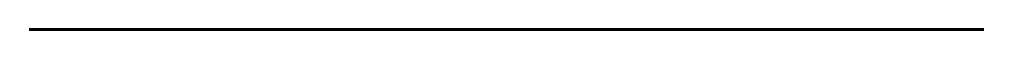
\begin{tikzpicture}
            \draw[very thick] (0,0) -- (\textwidth,0) {};
        \end{tikzpicture}\FloatBarrier\parindent 0pt
        \bfseries {\huge \sc{Building blocks for Finite Element computations in
                IPPL}}
        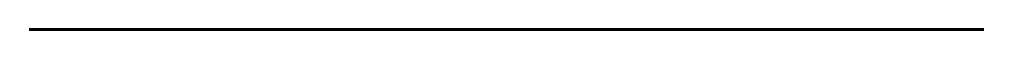
\begin{tikzpicture}
            \draw[very thick] (0,0) -- (\textwidth,0) {};
        \end{tikzpicture}}
    \author{
        \textsc{{{\LARGE Bachelor Thesis}}} \\[5pt]
        \small in Computational Science and Engineering \\[5pt]
        \small Department of Mathematics \\[5pt] \small ETH Zurich \vspace{0.4cm} \\[0.2in]
        \\ \small written by \\[5pt]
        %\small \sc{BSc ETH xxx} \\
        \sc{Lukas Bühler} \\
        \vspace{1cm} \\
        \small supervised by \\[5pt]
        Dr.\ A.\ Adelmann (ETH \& PSI)\\
        \vspace{0.5cm} \\
        \small scientific advisers \\[5pt]
        Sonali Mayani (PSI)\\
        Dr. M. Frey (University of St Andrews)\\
        Dr. S. Muralikrishnan (Jülich Supercomputing Center)\\
        \vspace{1.5cm} \\
        \today
    }
    \date{}
    % \clearpage
    \maketitle
    \thispagestyle{empty}
\end{titlepage}

\setcounter{page}{0}  % set page number -> such that table of contents is first page

%%%%%%%%%%%%%%%%%%%%%%%%%%%%%%%%%%%%%%%%%%%%%%%%%%%%%%%%%%%%%%%%%%%%%%%%%%%%%%%%%%%%%%%%%%%%%%%%%%%%%%%%%%%%%%%%%%%%%%%%%
% ABSTRACT
%%%%%%%%%%%%%%%%%%%%%%%%%%%%%%%%%%%%%%%%%%%%%%%%%%%%%%%%%%%%%%%%%%%%%%%%%%%%%%%%%%%%%%%%%%%%%%%%%%%%%%%%%%%%%%%%%%%%%%%%%

% \begin{abstract}

% \end{abstract}

%%%%%%%%%%%%%%%%%%%%%%%%%%%%%%%%%%%%%%%%%%%%%%%%%%%%%%%%%%%%%%%%%%%%%%%%%%%%%%%%%%%%%%%%%%%%%%%%%%%%%%%%%%%%%%%%%%%%%%%%
% TABLE OF CONTENTS
%%%%%%%%%%%%%%%%%%%%%%%%%%%%%%%%%%%%%%%%%%%%%%%%%%%%%%%%%%%%%%%%%%%%%%%%%%%%%%%%%%%%%%%%%%%%%%%%%%%%%%%%%%%%%%%%%%%%%%%%
\newpage
\pagenumbering{roman}
\tableofcontents


% 27.08.2015, http://tex.stackexchange.com/questions/11579/captions-for-figures-in-listoffigures

% 27.08.2015, https://www.sharelatex.com/learn/Lists_of_tables_and_figures
\listoffigures
%\listoftables
%\lstlistoflistings
% 06.09.2015, http://tex.stackexchange.com/questions/165903/optional-caption-in-listings-for-listoflistings

%\listofmyoutputs

\newpage
\pagenumbering{arabic}

%%%%%%%%%%%%%%%%%%%%%%%%%%%%%%%%%%%%%%%%%%%%%%%%%%%%%%%%%%%%%%%%%%%%%%%%%%

\chapter{Introduction}
\label{chapter:introduction}

Plasma, often referred to as the fourth state of matter, consists of a gas-like collection of
charged particles (ions and electrons) that exhibit a collective behavior.
Understanding its dynamics under the influence of electric and magnetic fields is of critical
importance for numerous areas in research as well as industry.
A prime example are non-neutral plasmas confined in particle accelerators where particle bunches are exposed to
a range of interesting phenomena which depend on the present plasma state.

In this report, we aim to model a phenomenon arising in ultra-cold plasmas where the transport of
the contained particles is strongly influenced by inter-particle collisions.
Modeling these scattering processes has been an active area of research for many decades
\cite{piwinski1974intra,kubo2001intrabeam}.
The individual scattering events are very weak and often happen over large distances.
Thus, modeling them as binary collisions requires very small timesteps which is not feasible for the
number of particles one usually encounters in dense plasmas.

Instead, researchers have explored methods emanating from plasma kinetic theory which model the scattering
processes via the Fokker-Planck (\gls{fp}) equation \cite{chandrasekhar1943,rosenbluth}.
It can be derived with a Taylor expansion of the statistically averaged effect on the velocity space due to
small-angle deflections. This effect describes advection (via friction) and diffusion in velocity space.
The definition of the friction and diffusion term of the \gls{fp} formalism is not straightforward, thus
researches usually have to state assumptions on the system state in order to approximate them
\cite{manheimer1997langevin,cadjan_ivanov_1999,jonesLangevin_1996}.
In our work we model the collisions via the Langevin formulation of the \gls{fp} equation \cite{cadjan_ivanov_1999}, allowing us to
model them as a stochastic process, providing a velocity dependent
deterministic friction and stochastic diffusion term \cite{stoel}.
This formulation facilitates the use of the Fokker-Planck term as part of the well-established
Particle-in-Cell (\gls{pic}) method \cite{bunemanPIC, dawsonPIC}.

\section{Motivation}

Free Electron Lasers (\gls{fel}) have the ability to generate beams that emit very short coherent light
pulses which exhibit wave lengths down to 0.1\ nm.
This laser is used, among many other applications, to map the atomic structure of proteins with a
high temporal resolution or allows investigating the atomic structure of crystalline matter.
An electron beam is emitted from an electron gun which is subsequently accelerated through an array
of magnets causing a lumping of the beam into bunches.
This process is prone to be negatively impacted by intra-beam scattering of the particles, causing the beam to widen
over time.
As this phenomenon negatively affects the achievable beam brightness, it is important to calibrate an
accelerator to counter this effect as much as possible.

Swiss\gls{fel} is an X-ray \gls{fel} at the Paul Scherrer Institute containing multiple beamlines for producing
many different types of X-ray pulses.
Prat et al. \cite{prat2022energy} have measured in experiments on this machine an energy spread for increased bunch
charges which is a magnitude larger than what their standard simulation codes predicted.
They showed that this blowup is caused mainly by intra-beam scattering and microbunching instabilities.
Being able to model the energy spread correctly is important as it directly influences how much
bunches can be compressed and also defines a lower bound on the achievable wavelength.
An existing method \cite{p3m_ulmer} based on the \gls{p3m} algorithm
(Particle-Particle Particle-Mesh, see Section \ref{section:PIC_method}) has been shown to model
intra-beam collisions adequately, but it does so at a considerable computational cost.
This inhibits simulating bunches over a complete beamline.
The aforementioned method of modeling collisions stochastically via the Langevin formulation promises
better computational complexity, therefore allowing to simulate larger number of particles and simulation domains.
We test the method on an experiment which is governed by disorder induced heating (\gls{dih}) \cite{mitchell2015parallel} and has been
shown to be resolved correctly only if individual particle collisions are considered (via the
\gls{p3m} method \cite{p3m_ulmer}).
This provides us with a challenging test case for the implemented method.

\section{Outline}

We start by introducing the notation used throughout the report, followed by a succinct treatise of the
underlying theory of plasma modeling in the context of kinetic theory, resulting in the Langevin formulation of
the \gls{fp} equation.
Subsequently we discuss the numerical methods used to solve the previously introduced equations and
propose an analytical test case that is used to verify the correctness of our implementation in the following chapter.
We then apply it to the physical test case governed by \gls{dih} and explore what
values the two collisional coefficients attain and how they impact the quantity of normalized emittance.
We conclude this work by highlighting the key findings of our investigation.
Additionally, we propose algorithmic improvements and suggest possible directions for further exploration
of the collisional terms applied in the context of \gls{dih}.


\chapter{Methodology}

For electromagnetic (EM) simulations, it is common to use the Finite Difference Time Domain (FDTD) scheme \cite{yee_finite-difference_1997}.
The FDTD scheme discretizes the time and space derivatives with central finite differences, hence, it only has 2nd-order accuracy.

Another method that can be used to solve the Maxwell equations is the Finite Element Method (FEM).
When solving EM problems with FEM, the space discretization is done using FEM
and other schemes such as Runge-Kutta methods are used to solve in the time domain.
This is known as Finite Element Time Domain (FETD).

FEM has multiple advantages compared to finite differences. It allows for more complex geometries
and higher-order elements (i.e.\ higher-order basis functions for the finite element spaces) to improve accuracy.
Using higher-order elements to improve the accuracy is known as $p$-refinement.
The higher-order elements allow FEM to achieve better accuracy without having to refine the mesh
and therefore improve the accuracy without really affecting the runtime, scalability and memory footprint.
It is also possible to refine the mesh, just as in the finite difference scheme,
which is known as $h$-refinement. It is even possible to do both with $hp$-refinement.

Furthermore, a matrix-free assembly algorithm can be used, which gives the method an even smaller memory footprint
and thus further improves the performance on GPUs.

In this work, we show an implementation of a Finite Element Method framework in IPPL \cite{frey_ippl-frameworkippl_2023}
with a matrix-free assembly algorithm and the possibility for $p$-refinement.



\section{Finite Element Method (FEM)}


\label{sec:fem_intro}

The Finite Element Method (FEM) is a method to solve partial differential equations (PDEs).
To use it, boundary value problems
need to be formulated into a variational boundary problem (weak form).
After that, the FEM consists of three main steps:
Firstly, discretizing or `meshing' the domain with a finite number of `elements'.
Secondly, approximating the solution of the PDE on each of the elements and finally
assembling the solutions from the elements in a linear system of equations (LSE).
This LSE can then be solved with any LSE solver.
FEM produces sparse problems,
which is why sparse LSE solvers are often used.
In this work, however, we use the conjugate gradient algorithm to solve the LSE instead,
since this allows us to avoid having to explicitly build the left-hand-side matrix (matrix-free).
For more details on the matrix-free method, see section \ref{sec:matrix_free}.

\subsection{Variational formulation}

\begin{definition}[Linear form]
    \label{def:linear_form}
    Given a vector space $V$ over $\R$, a \emph{linear form} $\ell$ is a mapping
    $\ell: V \mapsto \R$ that satisfies
    \cite[Def.~0.3.1.4]{hiptmair_numerical_2023}
    \begin{align}
        \ell(\alpha u + \beta v) = \alpha \ell(u) + \beta \ell(v), \quad
        \forall u,v \in V, \ \forall \alpha, \beta \in \R.
    \end{align}
\end{definition}

\begin{definition}[Bilinear form]
    \label{def:bilinear_form}
    Given a vector space $V$ over $\R$, a \emph{bilinear form} $\mathrm{a}$ on $V$
    is a mapping $\mathrm{a}: V \times V \mapsto \R$, for which it holds
    \cite[Def.~0.3.1.4]{hiptmair_numerical_2023}
    \begin{align}
         & \mathrm{a}\left(\alpha_1 v_1+\beta_1 u_1, \alpha_2 v_2+\beta_2 u_2\right)= \nonumber \\
         & \qquad \alpha_1 \alpha_2 \mathrm{a}\left(v_1, v_2\right)
        +\alpha_1 \beta_2 \mathrm{a}\left(v_1, u_2\right)
        +\beta_1 \alpha_2 \mathrm{a}\left(u_1, v_2\right)
        +\beta_1 \beta_2 \mathrm{a}\left(u_1, u_2\right),                                       \\
        \nonumber                                                                               \\
         & \forall u_i, v_i \in V, \alpha_i, \beta_i \in \mathbb{R}, i=1,2. \nonumber
    \end{align}
\end{definition}

\begin{definition}[Continuous Linear Form]
    \label{def:cont_linear_form}
    Given a normed vector space $V$ with norm $\|\cdot\|$, a linear form $\ell: V \to \R$
    is \emph{continuous} on $V$ if \cite[Def~1.2.3.42]{hiptmair_numerical_2023}
    \begin{align}
        \exists C > 0: \quad |\ell(v)| \leq C\|v\| \quad \forall v \in V,
    \end{align}
    holds for $C \in \R$.
\end{definition}
\begin{definition}[Continuous Bilinear Form]
    \label{def:cont_bilinear_form}
    Given a normed vector space $V$ with norm $\|\cdot\|$,
    a bilinear form $a: V \times V \to \R$ on $V$ is \emph{continuous}, if
    \cite[Def~1.2.3.42]{hiptmair_numerical_2023}
    \begin{align}
        \exists K > 0: \quad |\mathrm{a}(u, v)| \leq K\|u\| \|v\| \quad \forall u,v \in V_0,
    \end{align}
    holds for $K \in \R$.
\end{definition}

\begin{definition}[(Galerkin) Linear Variational Problem (LVP)]
    \label{def:lin_var_prob}
    We define a \emph{linear variational problem (LVP)} as
    \cite[Def.~1.4.1.7]{hiptmair_numerical_2023}
    \begin{align}
        u \in V: \quad \mathrm{a}(u, v) = \ell(v) \quad \forall v \in V, \label{eq:lin_var_prob}
    \end{align}
    where $V$ is a vector space, with norm $\|\cdot\|_V$,
    $\mathrm{a}: V \times V \mapsto \R$ is a continuous bilinear form and
    $\ell: V \mapsto \R$ is a continuous linear form.
    The function $u \in V$ is called the \emph{trial function} and the functions $v \in V$ are called the \emph{test functions}.

    In a generalized linear variational problem, the test and trial functions can be from different vector spaces, defined on the same subspace.
    Then these two vector spaces are called the test space and the trial space. However, in this work, we are only considering
    Galerkin Finite Element Methods where the test and the trial space are the same vector space, by definition.
\end{definition}

\subsubsection{Example: Poisson Equation}
\label{sec:poisson_eq}

The strong form of the Poisson equation with homogeneous Dirichlet boundary conditions is
\begin{align}
    \begin{array}{r l}
        -\Delta u = f & u \in \Omega,          \\
        u        = 0  & u \in \partial \Omega,
    \end{array}
    \label{eq:poisson_strong_form}
\end{align}
where $\Omega$ is the domain, $\partial \Omega$ is the boundary of the domain $\Omega$ and $f: \Omega \mapsto \R$ is the source function.

The weak-form or variational equation of the Poisson equation with homogeneous Dirichlet boundary conditions is
\begin{align}
    \int_\Omega \nabla u \cdot \nabla v \ d\vec{x} = \int_\Omega f v \ d\vec{x},
    \label{eq:poisson_weak_form}
\end{align}
where $v \in V$ is the test function and $u \in V$ is the trial function,
and $f: \Omega \to \R$ is the source function.
The derivation can be found in \cite{hiptmair_numerical_2023}.

The bilinear form and the linear of this problem are therefore
\begin{align}
    \mathrm{a}(u, v) & = \int_\Omega \nabla u \cdot \nabla v \ d\vec{x}, \\
    \ell(v)          & = \int_\Omega f v \ d\vec{x}.
\end{align}

\subsection{Discretization (Meshing)}

Recall the definition of the linear variational problem (Def. \ref{def:lin_var_prob}):

\begin{align}
    u \in V: \quad \mathrm{a}(u, v) = \ell(v) \quad \forall v \in V, \tag{\ref{eq:lin_var_prob}}
\end{align}

where $\mathrm{a}: V \times V \mapsto \R$ is the bilinear form and $\ell: V \mapsto \R$
is the linear form, $u$ is the trial function and $v$ are the test functions.

The first part of the discretization (meshing) step is the replacement of the
infinite-dimensional vector space $V$ in the linear variational problem with a
finite-dimensional subspace $V_{h} \subset V$ \cite[Chapter~2.2.1]{hiptmair_numerical_2023}.

\begin{definition}[Discrete (linear) variational problem (DVP)]
    \label{def:discrete_var_prob}
    The \emph{discrete variational problem (DVP)} is defined as
    \cite[Def.~2.2.1.1]{hiptmair_numerical_2023}
    \begin{align}
        \label{eq:discrete_var_eq}
        u_h \in V_{h}: \quad \mathrm{a}(u_h, v_h) = \ell(v_h), \quad \forall v_h \in V_{h},
    \end{align}
    where $u_h$ is the discretized trial function or \emph{Galerkin solution},
    $v_h$ are the discretized test functions, $\mathrm{a}: V_h \times V_h \to \R$
    is a continuous bilinear form and $\ell: V_h \to \R$ is a continuous linear form.
\end{definition}

The next step in the Galerkin Discretization is the definition of the basis
functions for the discrete variational problem.

We choose an ordered basis $\{b_h^1, \dots, b_h^N\}$ of $V_{h}$ with $N := \dim V_{h}$
where for every $v_h \in V_h$ there are unique coefficients $\nu_i \in \R, i \in \{ 1, \dots, N \}$,
such that $v_h = \sum_{i=1}^{N} \nu_i b_h^i$ \cite[Def.~0.3.1.2]{hiptmair_numerical_2023}.

Inserting this basis representation into the variaional equation \ref{eq:discrete_var_eq} yields:
\begin{align}
     & v_h \in V_{h} \Rightarrow v_h = \nu_1 b_h^1+\cdots+\nu_N b_h^N, \quad \nu_i \in \mathbb{R}, \\
     & u_h \in V_{h} \Rightarrow u_h = \mu_1 b_h^1+\cdots+\mu_N b_h^N, \quad \mu_i \in \mathbb{R},
\end{align}

where the number $N$ is the dimension of the discrete vector space $V_{h}$ and $\nu_i, \mu_i \in \R, \ i \in \{1, \dots, N\}$
are unique coefficients.

The basis functions also have to satisfy the cardinal basis property, as given by definition \ref{def:cardinal_basis_property}.

\begin{definition}[Cardinal basis property]
    \label{def:cardinal_basis_property}

    \begin{align}
        b_h^j(\vec{x}_i) = \begin{cases}
                               1 & i = j,      \\
                               0 & \text{else}
                           \end{cases}, \quad
        i,j \in \{ 1, ..., N \}.
    \end{align}
\end{definition}

Note: In this work, we refer to the basis functions on the global vector space as the
basis functions and to the basis functions restricted to an element $K$ as the
\emph{shape functions}.

\begin{definition}[Shape function]
    For an element $K$, we define the \emph{shape functions} as the basis functions,
    restricted to the element $K$:
    \begin{align}
        b^i_K := b^i_{h|K}.
    \end{align}
\end{definition}
Note: The letter $K$ for the shape function $b^i_K$ may be omitted where the context is clear.

Inserting the definitions of the basis functions into the variational equation %\cite[Chapter~2.2.2]{hiptmair_numerical_2023}
\begin{align}
    \mathrm{a}(u_h, v_h)                                                                                            & = \ell(v_h) \quad                                 & \forall u_h, v_h \in V_{0,h},                                   \\
    \sum_{k=1}^N \sum_{j=1}^N \mu_k \nu_j \, \mathrm{a}\left(b_h^k, b_h^j\right)                                    & = \sum_{j=1}^N \nu_j \ell\left(b_h^j\right) \quad & \forall \nu_1, \dots, \nu_N, \mu_1, \dots \mu_N \in \mathbb{R}, \\
    \sum_{j=1}^N \nu_j\left(\sum_{k=1}^N \mu_k \, \mathrm{a}\left(b_h^k, b_h^j\right)-\ell\left(b_h^j\right)\right) & = 0 \quad                                         & \forall \nu_1, \dots, \nu_N, \mu_1, \dots \mu_N \in \mathbb{R}, \\
    \sum_{k=1}^N \mu_k \, \mathrm{a}\left(b_h^k, b_h^j\right)                                                       & = \ell\left(b_h^j\right)                          & \text { for } j=1, \dots, N.
\end{align}

\begin{definition}[Stiffness matrix]
    \label{def:stiffness_mat}
    The stiffness matrix (or Galerkin matrix) is the matrix of the bilinear form evaluations
    defined as:
    \begin{align}
        \mat{A} = \left[ \mathrm{a}(b_h^j, b_h^i) \right]^N_{i,j=1}, \ \in \R^{N,N}.
        \label{eq:stiffness_mat}
    \end{align}
\end{definition}

\begin{definition}[Load vector]
    \label{def:load_vec}
    The load vector (or right-hand-side vector) is the vector of linear form evaluations
    defined as:
    \begin{align}
        \vec{\varphi} = \left[ \ell(b_h^i) \right]^N_{i=1} \in \R^{N}.
        \label{eq:load_vec}
    \end{align}
\end{definition}

To compute each entry of the stiffness matrix and load vector,
the integrals from the bilinear form and linear form are approximated.
This is done with numerical quadrature (numerical integration).

We arrive at the linear system of equations (LSE):

\begin{align}
    \mat{A}\vec{\mu} = \vec{\varphi}.
\end{align}




\section{Matrix-free Method for FEM computations}

\label{sec:matrix_free}

In 2017, Ljungkvist showed that matrix-free finite element algorithms
have many benefits on modern manycore processors and graphics cards (GPUs)
compared to alternative sparse matrix-vector products \cite{ljungkvist_matrix-free_2017}.
Additionally, in 2023, Settgast et.\ al showed that in the context of the
conjugate gradient (CG) method, the matrix-free approach compares favorably
even for low-order FEM \cite{settgast_performant_2023}.

Motivated by those findings, we chose to implement a matrix-free assembly algorithm that integrates
into the conjugate gradient algorithm, which is already implemented in IPPL.

The CG method is an iterative method and terminates once the norm of the residual is smaller than the specified tolerance $\epsilon \in \R_{>0}$.
The pseudocode for the CG algorithm in IPPL is given in Algorithm \ref{alg:conjugate_gradient}.


\begin{algorithm}[h]

    %\vspace{0.3cm}
    $\vec{x} \gets \text{initial guess, }(\text{usually }\vec{0})$

    $\vec{b} \gets \vec{\varphi}$

    $\vec{p} \gets \mat{A} \vec{x}$

    $\vec{r} \gets \vec{b} - \vec{p}$

    \While{$\|\vec{r}\|_2 < \epsilon$}{
        $\vec{z} \gets \mat{A}\vec{p}$

        \vspace{0.2cm}
        $\displaystyle \alpha \gets \frac{\vec{r}^\top \vec{r}}{\vec{p}^\top \vec{z}}$
        \vspace{0.2cm}

        $\vec{x} \gets \vec{x} + \alpha \vec{p}$

        $\vec{r}_\text{old} \gets \vec{r}$

        $\vec{r} \gets \vec{r} - \alpha \vec{z}$

        \vspace{0.2cm}
        $\displaystyle \beta \gets \frac{\vec{r}^\top \vec{r}}{\vec{r}_\text{old}^\top \vec{r}_\text{old}}$
        \vspace{0.2cm}

        $\vec{p} \gets \vec{r} + \beta \vec{p}$
    }
    \vspace{0.3cm}
    \caption{Pseudocode of the CG algorithm implemented in IPPL.}
    \label{alg:conjugate_gradient}
\end{algorithm}

In the CG method, the stiffness matrix $\mat{A}$ is used in the initialization and in the while loop itself, and in both cases, it is multiplied with a vector.
The implemented FEM framework provides an assembly function to replace this matrix-vector product $\mat{A}\vec{x}$.
The assembly function will return the same resulting vector, but without building the full stiffness matrix $\mat{A}$, thus being ``matrix-free''.

More detailed information regarding the implementation of this assembly algorithm is given in section \ref{sec:assembly}.



\section{Independent Parallel Particle Layer (IPPL)}

The Independent Parallel Particle Layer (IPPL) \cite{frey_ippl-frameworkippl_2023} \cite{muralikrishnan_scaling_2022}
is a performance portable \texttt{C++} library for Particle-Mesh methods.
It is a portable, massively parallel toolkit using the Message Passing Interface (MPI) for inter-processor communication,
HeFFTe \cite{ayala_heffte_2020} as a Fast Fourier Transform (FFT) library and Kokkos \cite{carter_edwards_kokkos_2014} for hardware portability.

\section{Arguments against using an external FEM library}

The Finite Element Method has been studied in great detail already and has been implemented for many languages, environments and use cases.
There are also many \texttt{C++} FEM libraries, for example, MFEM \cite{anderson_mfem_2021} and deal.II \cite{bangerth_dealiigeneral-purpose_2007}.

The possibility of interfacing IPPL with an external library to introduce the Finite Element Method was considered,
but it was decided against for several reasons.
Firstly, new dependencies can bring problems in the future and they further complicate the compilation and installation of IPPL.
Secondly, almost all external libraries use non-standard or custom datatypes.
Since the performance of IPPL on supercomputers is very important, it is crucial to avoid data copies,
which would occur when using a different data type to support an external library,
as they incur high data movement costs, especially on GPUs.

\section{Focus and Scope of this Thesis}

The focus of this Bachelor thesis is the software design and implementation
of the building blocks for the Finite Element Method in the IPPL \cite{frey_ippl-frameworkippl_2023} library.
The focus was on structured, rectilinear grids with rectangular hexahedral (``brick'') elements and the possibility for $p$-refinement.

The term `building blocks' refers to the different parts that are necessary for a functioning FEM implementation.
For example, a class for numerical integration (quadrature),
classes for mesh and degree of freedom (DOF) index mapping and assembly functions for building the resulting linear system of equations.

The framework implemented in this thesis supports first-order Lagrangian finite elements in
one to three dimensions with a matrix-free assembly function that interfaces directly into the CG algorithm.
It supports the basic midpoint quadrature rule and the polynomial Gauss-Jacobi quadrature rule.
For essential boundary conditions, only homogeneous Dirichlet boundary conditions are supported at the moment.

Additionally, a solver to solve the Poisson equation was implemented as a proof-of-concept.



\chapter{Implementation}

In this chapter, the first section (\ref{sec:software_architecture}) will go into the general organization
and software architecture of the FEM framework in IPPL. The following sections will go into the specifics
of the FEM building blocks and their implementation.

\section{Software Architecture}
\label{sec:software_architecture}

From a software architecture perspective, the FEM framework was designed to have high modularity
and is easily extensible as a result.
A quick overview is given in the Unified Modeling Language (UML) diagram in figure \ref{fig:software_arch_uml}.

The main interface for all the building blocks is the abstract \texttt{FiniteElementSpace} class.
It has a reference to the mesh, the reference element and the quadrature rule that is used in the assembly.

The IPPL \texttt{Mesh} class is abstract as well and other mesh classes like the IPPL \texttt{UniformMesh} class inherit from it.
At the moment, only rectilinear meshes are supported in IPPL.

The reference element class is abstract and it defines the transformation functions. It has pure virtual
functions to force its child classes to implement the functions to support these transformations.
Implemented classes that inherit from it are the \texttt{EdgeElement}, \texttt{QuadrilateralElement} and \texttt{HexahedralElement} classes.

The \texttt{Quadrature} class is also abstract and implements the functions for transforming 1D quadrature
weights and nodes to tensor product quadrature nodes and weights on the reference elements.
At the moment there are two different quadrature rules implemented that inherit from the
\texttt{Quadrautre} base class. The \texttt{MidpointQuadrature} rule that was implemented for testing and
the \texttt{GaussJacobiQuadrature} class which implements the Gauss-Jacobi quadrature rule.

The \texttt{LagrangeSpace} class inherits from the abstract \texttt{FiniteElementSpace} base class
and defines the degree of freedom (DOF) operations and assembly functions for the Lagrangian finite elements.

The \texttt{FEMSolver} class is used to showcase the FEM framework.
It solves the Poisson equation using first-order Lagrangian finite element methods
with the existing conjugate gradient algorithm from IPPL and the Gauss-Jacobi quadrature rule.

\begin{figure}[h]
    \centering
    \resizebox{\hsize}{!}{%
        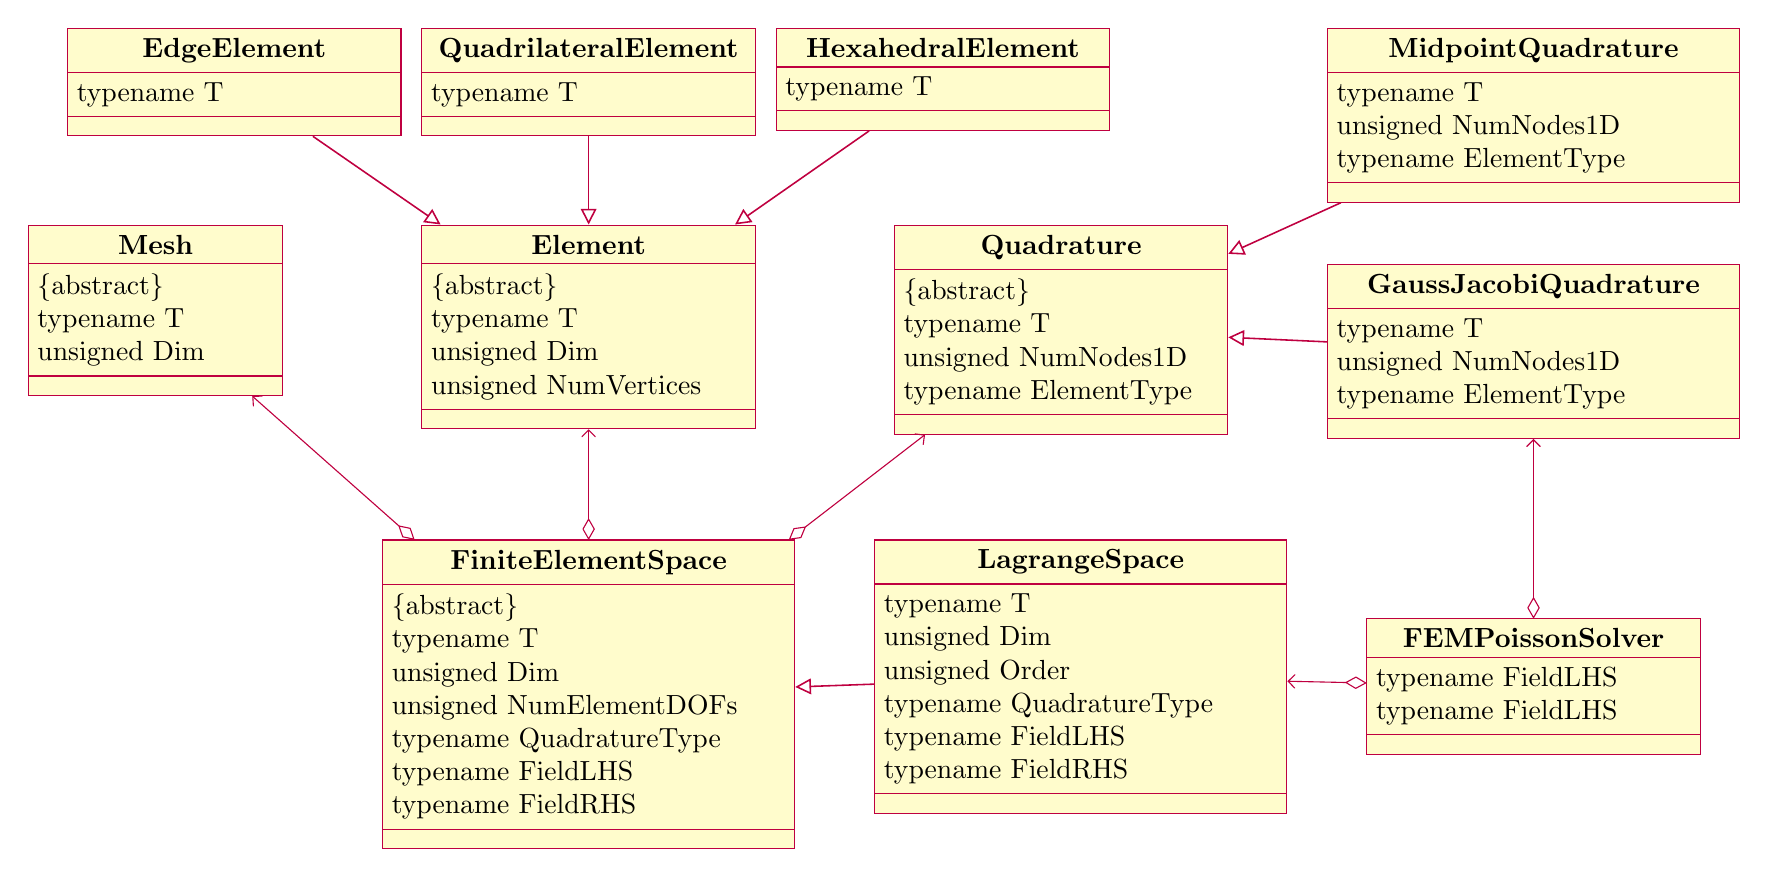
\begin{tikzpicture}

            \begin{class}[text width=5cm]{FiniteElementSpace}{0,0}
                \attribute{\{abstract\}}
                \attribute{typename T}
                \attribute{unsigned Dim}
                \attribute{unsigned NumElementDOFs}
                \attribute{typename QuadratureType}
                \attribute{typename FieldLHS}
                \attribute{typename FieldRHS}
            \end{class}

            \begin{class}[text width=5cm]{LagrangeSpace}{6.25,0}
                \attribute{typename T}
                \attribute{unsigned Dim}
                \attribute{unsigned Order}
                \attribute{typename QuadratureType}
                \attribute{typename FieldLHS}
                \attribute{typename FieldRHS}
            \end{class}
            \draw[-{Triangle[length=2mm,width=2mm,fill=white]}, umlcolor, line width=0.2mm] (LagrangeSpace) -- (FiniteElementSpace);

            \begin{class}[text width=3cm]{Mesh}{-5.5, 4}
                \attribute{\{abstract\}}
                \attribute{typename T}
                \attribute{unsigned Dim}
            \end{class}
            \aggregation{FiniteElementSpace}{}{}{Mesh}

            % ELEMENTS

            \begin{class}[text width=4cm]{Element}{0, 4}
                \attribute{\{abstract\}}
                \attribute{typename T}
                \attribute{unsigned Dim}
                \attribute{unsigned NumVertices}
            \end{class}
            \aggregation{FiniteElementSpace}{}{}{Element}

            \begin{class}[text width=4cm]{EdgeElement}{-4.5, 6.5}
                \attribute{typename T}
            \end{class}
            \draw[-{Triangle[length=2mm,width=2mm,fill=white]}, umlcolor, line width=0.2mm] (EdgeElement) -- (Element);

            \begin{class}[text width=4cm]{QuadrilateralElement}{0, 6.5}
                \attribute{typename T}
            \end{class}
            \draw[-{Triangle[length=2mm,width=2mm,fill=white]}, umlcolor, line width=0.2mm] (QuadrilateralElement) -- (Element);

            \begin{class}[text width=4cm]{HexahedralElement}{4.5, 6.5}
                \attribute{typename T}
            \end{class}
            \draw[-{Triangle[length=2mm,width=2mm,fill=white]}, umlcolor, line width=0.2mm] (HexahedralElement) -- (Element);

            % QUADRATURE

            \begin{class}[text width=4cm]{Quadrature}{6, 4}
                \attribute{\{abstract\}}
                \attribute{typename T}
                \attribute{unsigned NumNodes1D}
                \attribute{typename ElementType}
            \end{class}
            \aggregation{FiniteElementSpace}{}{}{Quadrature}

            \begin{class}[text width=5cm]{GaussJacobiQuadrature}{12, 3.5}
                \attribute{typename T}
                \attribute{unsigned NumNodes1D}
                \attribute{typename ElementType}
            \end{class}
            \draw[-{Triangle[length=2mm,width=2mm,fill=white]}, umlcolor, line width=0.2mm] (GaussJacobiQuadrature) -- (Quadrature);

            \begin{class}[text width=5cm]{MidpointQuadrature}{12, 6.5}
                \attribute{typename T}
                \attribute{unsigned NumNodes1D}
                \attribute{typename ElementType}
            \end{class}
            \draw[-{Triangle[length=2mm,width=2mm,fill=white]}, umlcolor, line width=0.2mm] (MidpointQuadrature) -- (Quadrature);

            % SOLVER

            \begin{class}[text width=4cm]{FEMPoissonSolver}{12,-1}
                \attribute{typename FieldLHS}
                \attribute{typename FieldLHS}
            \end{class}
            \aggregation{FEMPoissonSolver}{}{}{LagrangeSpace}
            \aggregation{FEMPoissonSolver}{}{}{GaussJacobiQuadrature}

        \end{tikzpicture}%
    }
    \caption{Software architecture of the FEM framework, showing the classes with their template arguments.}
    \label{fig:software_arch_uml}
\end{figure}


\begin{figure}[h]
    \dirtree{%
        .1 ippl/.
        % .2 doc/.
        .2 src/.
        .3 FEM/.
        .4 Elements/.
        .5 EdgeElement.h.
        .5 EdgeElement.hpp.
        .5 Element.h.
        .5 Element.hpp.
        .5 HexahedralElement.h.
        .5 HexahedralElement.hpp.
        .5 QuadrilateralElement.h.
        .5 QuadrilateralElement.hpp.
        .4 Quadrature/.
        .5 GaussJacobiQuadrature.h.
        .5 GaussJacobiQuadrature.hpp.
        .5 MidpointQuadrature.h.
        .5 MidpointQuadrature.hpp.
        .5 Quadrature.h.
        .5 Quadrature.hpp.
        .4 CMakeLists.txt.
        .4 FiniteElementSpace.h.
        .4 FiniteElementSpace.hpp.
        .4 LagrangeSpace.h.
        .4 LagrangeSpace.hpp.
        % .2 test/.
        % .3 FEM/.
        % .3 solver/.
        % .4 TestFEMPoissonSolver.cpp.
        % .2 unit\_test/.
        % .3 FEM/.
        % .4 CmakeLists.txt.
        % .4 EdgeElement.cpp.
        % .4 FiniteElementSpace.cpp.
        % .4 GaussJacobiQuadrature.cpp.
        % .4 LagrangeSpace.cpp.
        % .4 MidpointQuadrature.cpp.
        % .4 Quadrature.cpp.
        % .4 QuadrilateralElement.cpp.
    }

    \caption{IPPL FEM framework source file structure.}
\end{figure}

\clearpage
\section{Finite Element Spaces, Meshes and Indexing}

To implement the Finite Element Method, functions are needed to map mesh vertices to elements and vice-versa.
In our implementation, this is implemented in the \texttt{FiniteElementSpace} class. It is also the base
class for the \texttt{LagrangeSpace} class that implements Lagrangian finite elements.
The \texttt{FiniteElementSpace} class is an abstract class that implements the mesh helper functions and also declares pure virtual member
functions for degree-of-freedom, reference element shape function evaluations and assembly functions.

\subsection{Mesh vertex and element index mapping}

At this time, IPPL implements only structured, rectilinear grid meshes.
In FEM, each mesh cell is assigned an element. The elements are indexed starting from zero (\texttt{C++} indexing)
in this implementation.

To define the position of a vertex in the structured rectilinear grid mesh,
we define a vector that has $N$ entries for an $N$ dimensional mesh with each entry representing
the position of a mesh cell in the $n$-th dimension.
In the implementation, the type alias for this vector is called \texttt{NDIndex},
following the naming convention from IPPL.

For example, in figure \ref{fig:mesh} the \texttt{NDIndex} of vertex $13$ would be $(3, 2)$.
The element \texttt{NDIndex} of $(3,1)$ corresponds to the element with index $7$.

Figure \ref{fig:mesh} illustrates the mesh vertex indexing (black) and element indexing (red).
Each vertex index is associated with the vertex \texttt{NDIndex},
as well as each element associated with the element \texttt{NDIndex}.

\begin{figure}[h]
    \centering
    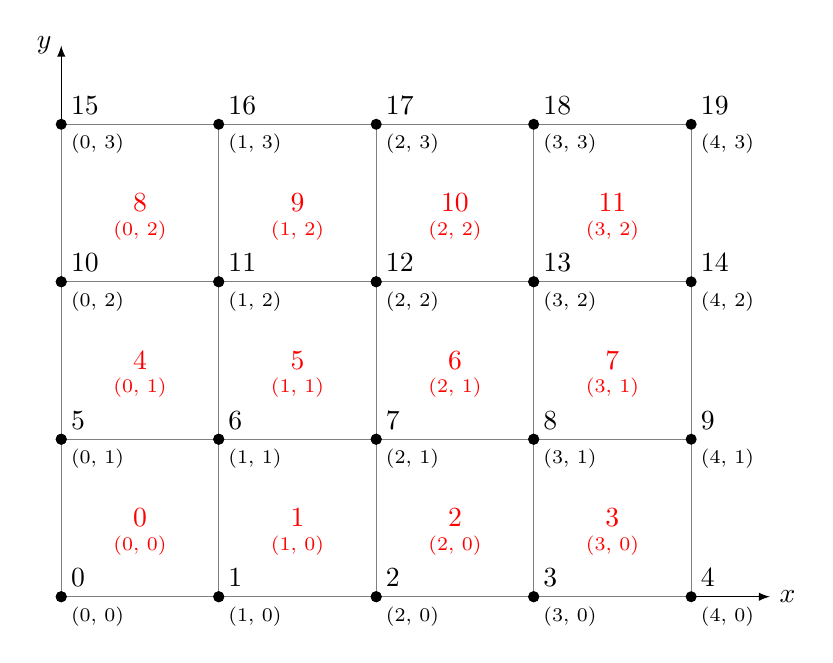
\begin{tikzpicture}
        \draw[-latex] (0,0) -- (9,0) node[right] {$x$};
        \draw[-latex] (0,0) -- (0,7) node[left] {$y$};

        % Draw grid over highlighted cells
        \draw[step=2cm,gray,very thin] (0,0) grid (8,6);

        % Mesh vertices
        \foreach \x in {0,1,2,3,4} {
                \foreach \y in {0,1,2,3} {
                        \fill (2*\x,2*\y) circle (2pt);
                        \pgfmathtruncatemacro\index{5*\y + \x}
                        \node[black, anchor=south west] at (2*\x,2*\y) {\index};
                        \node[black, font=\scriptsize, anchor=north west] at (2*\x,2*\y) {(\x, \y)};
                    }
            }

        % Elements
        \foreach \x in {0,1,2,3} {
                \foreach \y in {0,1,2} {
                        \fill (2*\x,2*\y) circle (2pt);
                        \pgfmathtruncatemacro\index{4*\y + \x}
                        \node[red] at (2*\x+1, 2*\y+1) {\index};
                        \node[red, font=\scriptsize, anchor=north] at (2*\x+1, 2*\y+0.9) {(\x, \y)};
                    }
            }
    \end{tikzpicture}

    \caption{Illustration of mesh vertex indexing and element indexing.}
    \label{fig:mesh}
\end{figure}

\subsection{The FiniteElementSpace Class}

The \texttt{FiniteElementSpace} class takes in template arguments for the floating point type \texttt{T},
the dimension \texttt{Dim} and the number of degrees of freedom on a reference element \texttt{NumElementDOFs}
the quadrature rule type \texttt{QuadratureType} and the two types for the left-hand-side IPPL \texttt{Field} and the right-hand-side IPPL \texttt{Field}.

This class declares additional pure virtual member functions in the header file, that child classes
need to define. These functions are for degrees of freedom, reference element shape functions evaluations and assembly operations and they
will be introduced in section \ref{sec:lagrange_class}.



\section{Elements and Transformations}
\label{sec:elements}
\subsection{Defining the Reference Elements}

In this section the three basic reference elements, for one, two and three dimensions, are defined.
They could be described as n-cuboid shapes because they are shaped like the cells of rectilinear structured grids.
For consistency with the implementation, the indices start at zero (\texttt{C++} indexing).

\subsubsection{Edge Element (1D)}

In a one-dimensional mesh, an element is a line segment or an edge.
The reference edge element is one-dimensional and starts at 0 and ends at 1.
The first vertex with index 0 is at $0$, and the second vertex with index 1 is at $1$.
the indexing is visualized in figure \ref{fig:edge_element}.

\begin{figure}[h]
    \vspace{0.5cm}
    \centering
    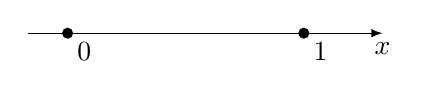
\begin{tikzpicture}
        \draw[-latex] (-0.5,0,0) -- (4,0,0) node[below] {$x$};

        % Define the vertices of the cube
        \coordinate (A) at (0, 0);
        \coordinate (B) at (3, 0);

        % Draw the edges of the cube
        \draw[black] (A) -- (B) -- cycle;

        % Draw the vertices of the cube
        \fill[black] (A) circle (2pt);
        \fill[black] (B) circle (2pt);

        % Label the vertices
        \node[below right] at (A) {0};
        \node[below right] at (B) {1};
    \end{tikzpicture}
    \caption{Illustration of the local vertex numbering on the reference edge element (1D).}
    \label{fig:edge_element}
\end{figure}

\subsubsection{Quadrilateral Element (2D)}

The 2D structured grid cells can be described by a quadrilateral. For rectilinear grids
those cells are rectangular.
However, the quadrilateral reference element in this framework aims to describe quadrilaterals,
which include parallelograms and by definition every closed, non-degenerate shape with four vertices.

The local vertices are ordered according to the right-hand rule.
The first vertex of the reference element is at $(0,0)$ and has index 0.
The second vertex of the reference element is located at $(1,0)$ and has index 1.
The vertex with index 2 is at $(1, 1)$ and the last vertex with index 3 is at $(0,1)$.
See figure \ref{fig:quad_element} for an illustration of the vertex indexing.

\begin{figure}[h]
    \centering
    \begin{tikzpicture}
        \draw[-latex] (-0.5,0,0) -- (4,0,0) node[below] {$x$};
        \draw[-latex] (0,-0.5,0) -- (0,4,0) node[above right] {$y$};

        % Define the vertices of the cube
        \coordinate (A) at (0, 0);
        \coordinate (B) at (3, 0);
        \coordinate (C) at (3, 3);
        \coordinate (D) at (0, 3);

        % Draw the edges of the cube
        \draw[black] (A) -- (B) -- (C) -- (D) -- cycle;

        % Draw the vertices of the cube
        \fill[black] (A) circle (2pt);
        \fill[black] (B) circle (2pt);
        \fill[black] (C) circle (2pt);
        \fill[black] (D) circle (2pt);

        % Label the vertices
        \node[below right] at (A) {0};
        \node[below right] at (B) {1};
        \node[below right] at (C) {2};
        \node[below right] at (D) {3};
    \end{tikzpicture}
    \caption{Illustration of the local vertex numbering on a quadrilateral element (2D).}
    \label{fig:quad_element}
\end{figure}

\subsubsection{Hexahedral Element (3D)}

Three-dimensional structured grids have hexahedral grid cells.
In rectilinear structured grids from IPPL, the cells can be described as bricks or rectangular cuboids.
The indexing follows the indexing from FEMSTER \cite{castillo_femster_2005}.
See figure \ref{fig:hex_element} for an illustration.

\begin{figure}[h]
    \centering
    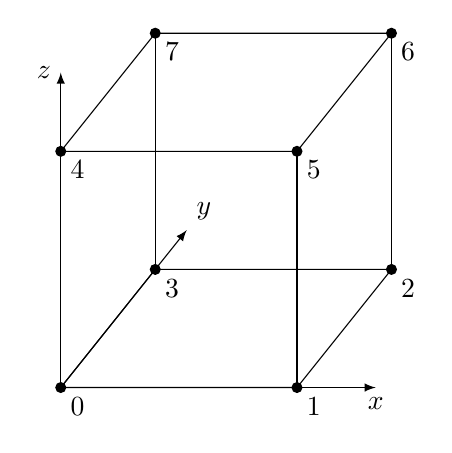
\begin{tikzpicture}[x={(1cm,0cm)}, y={(0.4cm,0.5cm)}, z={(0cm,1cm)}]
        \draw[-latex] (0,0,0) -- (4,0,0) node[below] {$x$};
        \draw[-latex] (0,0,0) -- (0,4,0) node[above right] {$y$};
        \draw[-latex] (0,0,0) -- (0,0,4) node[left] {$z$};

        % Define the vertices of the cube
        \coordinate (A) at (0, 0, 0);
        \coordinate (B) at (3, 0, 0);
        \coordinate (C) at (3, 3, 0);
        \coordinate (D) at (0, 3, 0);
        \coordinate (E) at (0, 0, 3);
        \coordinate (F) at (3, 0, 3);
        \coordinate (G) at (3, 3, 3);
        \coordinate (H) at (0, 3, 3);

        % Draw the edges of the cube
        \draw[black] (A) -- (B) -- (C) -- (D) -- cycle;
        \draw[black] (E) -- (F) -- (G) -- (H) -- cycle;
        \draw[black] (A) -- (E);
        \draw[black] (B) -- (F);
        \draw[black] (C) -- (G);
        \draw[black] (D) -- (H);

        % Draw the vertices of the cube
        \fill[black] (A) circle (2pt);
        \fill[black] (B) circle (2pt);
        \fill[black] (C) circle (2pt);
        \fill[black] (D) circle (2pt);
        \fill[black] (E) circle (2pt);
        \fill[black] (F) circle (2pt);
        \fill[black] (G) circle (2pt);
        \fill[black] (H) circle (2pt);

        % Label the vertices
        \node[below right] at (A) {0};
        \node[below right] at (B) {1};
        \node[below right] at (C) {2};
        \node[below right] at (D) {3};
        \node[below right] at (E) {4};
        \node[below right] at (F) {5};
        \node[below right] at (G) {6};
        \node[below right] at (H) {7};
    \end{tikzpicture}
    \caption{Illustration of the local vertex numbering on a hexahedral element (3D).}
    \label{fig:hex_element}
\end{figure}

\subsection{Transformations}
\label{sec:transformations}

In order to compute the values of the shape functions on the reference element $\hat{K}$
and transform them back to the global element $K$, we need a function that maps the global element to the reference element.
For this, we define the transformation function $\mat{\Phi}_K$ below.

\begin{definition}[Transformation Function]
    The transformation function  $\mat{\Phi}_K$ maps points from the local coordinate system of the reference element $\hat{K}$ to
    the global coordinate system of the global element $K$:
    \begin{align}
        \mat{\Phi}_K: \hat{K} \mapsto K.
    \end{align}
    To transform a point $\hat{\vec{x}} \in \hat{K}$ to its point in the global coordinate system $\vec{x} \in K$ we use:
    \begin{align}
        \vec{x} & = \mat{\Phi}_K(\hat{\vec{x}}).
    \end{align}
    This is called a local-to-global transformation.

    The opposite from $\vec{x} \in K$ to $\hat{\vec{x}} \in \hat{K}$ is the global-to-local transformation using the inverse
    of the transformation function $\mat{\Phi}^{-1}_K$:
    \begin{align}
        \hat{\vec{x}} & = \mat{\Phi}^{-1}_K(\vec{x}).
    \end{align}
\end{definition}

At the time of writing, IPPL only supports rectilinear structured grid meshes for which affine transformations are sufficient.
Thus, only affine transformations were implemented, instead of more general bilinear transformations.
For more information on how to update this implementation to use bilinear transformations instead, see
section \ref{sec:bilinear_transformations} in the Appendix.

The difference between the bilinear and affine transformations is that the affine transformations can only
handle transformations to parallelograms whereas bilinear transformations cover all possible transformations for quadrilaterals.

\begin{definition}[Affine Transformation]
    \label{def:affine_trans}
    An affine transformation combines a linear transformation and a translation and is defined as
    \begin{align}
        \mat{\Phi}_K(\hat{\vec{x}}) = \mat{F}_K \hat{\vec{x}} + \vec{\tau}_K,
    \end{align}
    where $\hat{\vec{x}}$ is the point to transform in the reference coordinate system, $\mat{F}_K$ is
    the transformation matrix and $\vec{\tau}_K$ is the translation vector.
\end{definition}

Also, on a side note, not implementing bilinear transformations means that technically the \texttt{QuadrilateralElement} class currently only supports
parallelograms instead of all quadrilaterals.
Similarly, the \texttt{HexahedralElement} does not support transformations to all hexahedrons.

Also, since we assume rectilinear grids, we can go one step further because the linear transformation in the affine transformation
can be simplified even more to just a scaling transformation.
Thus we can use a transformation matrix as follows:
\begin{align}
    \label{eq:scaling_transform_mat}
    \mat{F}_K := \begin{bmatrix}
                     \boldsymbol{v}^1_x - \boldsymbol{v}^0_x & 0                                       & 0                                       \\
                     0                                       & \boldsymbol{v}^2_y - \boldsymbol{v}^0_y & 0                                       \\
                     0                                       & 0                                       & \boldsymbol{v}^4_z - \boldsymbol{v}^0_z
                 \end{bmatrix}.
\end{align}
Equation \ref{eq:scaling_transform_mat} is the scaling transformation matrix for three dimensions,
where $\vec{v}^i \in \R^d$ is the $i$-th local vertex of the element with $d$ entries for each dimension.

\begin{figure}[h]
    \centering
    \begin{tikzpicture}

        \draw[->] (0,0) -- (2.4,0) node[at end, right] {$\hat{x}$};
        \draw[->] (0,0) -- (0,2.4) node[at end, above] {$\hat{y}$};
        \draw[step=2cm,black,thin] (0,0) grid (2,2);
        \node[black, font=\small] at (1,1) {$\hat{K}$};

        \draw[->] (3,1.5) -- (5,1.5) node[midway, above] {$\mat{\Phi}_K$};
        \draw[->] (5,1) -- (3,1) node[midway, below] {$\mat{\Phi}^{-1}_K$};

        \draw[step=2cm,gray,very thin] (6,0) grid (12.4,5.4);
        \draw[->] (6,0) -- (12.4,0) node[at end, right] {$x$};
        \draw[->] (6,0) -- (6,5.4) node[at end, above] {$y$};

        \draw[thin,black] (7.8,1.2) -- (11,1.2);
        \draw[thin,black] (11,1.2) -- (11,3.6);
        \draw[thin,black] (7.8,1.2) -- (7.8,3.6);
        \draw[thin,black] (7.8,3.6) -- (11,3.6);
        \node[black, font=\small] at (9.9,2.4) {$K$};

        \fill[black] (7.8,1.2) circle (1.5pt);
        \node[black, font=\small, anchor=north west] at (7.8,1.2) {$\vec{v}^0$};
        \fill[black] (11,1.2) circle (1.5pt);
        \node[black, font=\small, anchor=north west] at (11,1.2) {$\vec{v}^1$};
        \fill[black] (7.8,3.6) circle (1.5pt);
        \node[black, font=\small, anchor=north west] at (7.8,3.6) {$\vec{v}^2$};
        \fill[black] (11,3.6) circle (1.5pt);
        \node[black, font=\small, anchor=north west] at (11,3.6) {$\vec{v}^3$};

        \draw[->] (6,0) -- (7.8,1.2) node[midway, above] {$\vec{\tau}_K\,$};
    \end{tikzpicture}
    \caption{Illustration of a 2D transformation (scaling and translation only).}
    \label{fig:affine_trans}
\end{figure}


\subsubsection{Applying Affine Tranformations}

In this subsection, the transformation will be applied to integrals and gradients.

First, we define how to apply the transformation to functions using the \emph{pullback} operation.

\begin{definition}[Pullback]
    The pullback $\mat{\Phi}_K^* f$ of a function $f$ is defined as \cite{hiptmair_numerical_2023}:

    \begin{align}
        \label{}
        (\mat{\Phi}_K^* f)(\hat{\vec{x}}) := f(\mat{\Phi}_K(\hat{\vec{x}})), \quad \hat{\vec{x}} \in \hat{K}.
    \end{align}

    It applies the transformation function $\mat{\Phi}_K$ to the input of the function $f$.
\end{definition}

\begin{definition}[Transformation Jacobian]
    The \emph{Transformation Jacobian} is defined as \cite{hiptmair_numerical_2023}:
    \begin{align}
        \mathbf{D\Phi}_K(\hat{\boldsymbol{x}})
        = \left[ \frac{\partial (\mathbf{\Phi}_K(\hat{\boldsymbol{x}}))_i}{\partial \boldsymbol{x}_j} \right]^d_{i,j = 1}.
    \end{align}
\end{definition}

In this work, with the simplifications applied from before, the Jacobian $\mat{D \Phi}_K$ is equal to the transformation matrix:
\begin{align}
    \mathbf{D\Phi}_K(\hat{\boldsymbol{x}}) = \mat{F}_K.
\end{align}

The pullback can be applied to the gradient of a function as follows:

\begin{align}
    \mat{\Phi}_{K}^{*}(\nabla_{\vec{x}} u)(\hat{\vec{x}})
     & = (\mat{D \Phi}_{K}(\hat{\vec{x}}))^{-\top}(\nabla_{\hat{\vec{x}}}(\mat{\Phi}^{*}_K u))(\hat{\vec{x}}) \\
     & = (\mat{D \Phi}_{K}(\hat{\vec{x}}))^{-\top}(\nabla_{\hat{\vec{x}}}u)(\mat{\Phi}_K(\hat{\vec{x}})),
\end{align}
with the notation: $\mat{S}^{-\top} := (\mat{S}^{-1})^\top = (\mat{S}^\top)^{-1}$.

Also, the inverse of the Transformation Jacobian is equal to the inverse of the transformation matrix:
\begin{align}
    \mathbf{D\Phi}_K^{-1}(\hat{\boldsymbol{x}}) = \mat{F}_K^{-1}.
\end{align}

The determinant of the Transformation Jacobian is therefore also equal to the determinant of the transformation matrix:

\begin{align}
    |\det \mathbf{D\Phi}_K(\hat{\boldsymbol{x}})| = |\det \mat{F}_K|.
\end{align}

\subsection{Element classes}

The \texttt{Element} class is the base class for all the reference elements.
The reference element classes that inherit from it, define the indexing and position of the local vertices.
They also define the transformation functions for the local-to-global transformations.

The base \texttt{Element} class is abstract and dimension-independent and it takes in arguments for the
dimension \texttt{Dim}, as well as the datatype \texttt{T} and the number of
vertices \texttt{NumVertices}. The number of vertices is required at compile time
to define the size of the IPPL Vector, which also takes the size as a template
argument at compile time.

For now, transformations to lower dimensions are not supported.
Therefore the dimension template argument has to have the same dimension as the mesh.

\section{Lagrangian Finite Element Methods}

\label{sec:lagrange}

In this work, we are looking at Lagrangian FEM on structured rectilinear grids,
also known as Tensor-Product Lagrangian FEM \cite{hiptmair_numerical_2023}.

The Lagrangian finite element space defines a set of piecewise continuous
polynomials of degree $p$ over the mesh. They are only piecewise over the element boundaries.

\begin{definition}[(Tensor-product) Lagrangian finite element spaces]
    We define the space of $p$-th degree
    Lagrangian finite element functions on a tensor product mesh $\mathcal{M}$ as \cite{hiptmair_numerical_2023}:
    \begin{align}
        \mathcal{S}_p^0(\mathcal{M}) := \{ v \in C^0(\bar{\Omega}):
        v_{|K} \in \mathcal{Q}_p(K) \ \forall K \in \mathcal{M}\},
    \end{align}
    where $\bar{\Omega}$ is the domain of the mesh, including the boundary,
    $\mathcal{Q}_p(K)$ is the set of basis functions that are tensor products of polynomials of degree $p$ spanning the element $K$
    and $v_{|K}$ are the functions $v$ restricted to element $K$.

    The space $\mathcal{S}_p^0$ contains continuous, piecewise polynomial functions
    that are made up of ``stitched together'' basis functions functions from the elementes in mesh $\mathcal{M}$.
\end{definition}

\subsection{Lagrangian shape functions}

Together with the Lagrangian finite element space, the basis functions have to be defined as well.
The basis functions are defined according to the policy of interpolation nodes through the cardinal
basis property (see def. \ref{def:cardinal_basis_property}).

\begin{definition}[Lagrange Polynomials]
    Given a set $\{ x_0, ..., x_n\} \subset \R$ of nodes, the \emph{Lagrange polynomials} are \cite{hiptmair_numerical_2020}
    \begin{align}
        L_i(x) := \prod_{j=0, j\neq i}^n \frac{x - x_i}{x_i - x_j}, \quad i=0, ..., n.
    \end{align}
\end{definition}

The Lagrange interpolating polynomial is the unique
polynomial of the lowest degree that interpolates a set of points \cite{hiptmair_numerical_2020}.
They satisfy the cardinal basis property on the interpolation nodes.

To define polynomial functions of degree $p$ on the elements, Lagrangian FEM utilizes
Lagrangian polynomials, hence the name.
We have a fixed number of degrees of freedom (DOFs) per element that correspond to the
local shape functions of the element.
The shape functions satisfy the cardinal basis property that they evaluate to one
at the location of the corresponding DOF and to zero at the locations of all the other DOFs.

\subsubsection{First-order shape functions}

In one dimension, first-order Lagrangian shape functions are polynomials of degree 1,
or linear polynomials, and interpolate two points.
The basis functions for first-order Lagrangian FEM are the well-known tent functions \cite{hiptmair_numerical_2023}.
The shape functions are:

\begin{align}
    \hat{b}^i(x) = \begin{cases}
                       1 - x & i=0, \\
                       x     & i=1.
                   \end{cases}
\end{align}

See figure \ref{fig:1_lagrange_1d} for a plot of 1D first-order Lagrangian shape functions.

\begin{figure}[h]
    \centering
    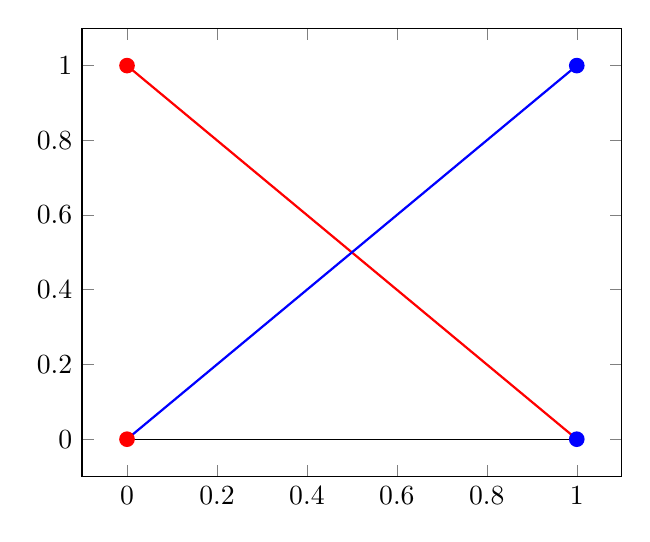
\begin{tikzpicture}
        \begin{axis}[domain=0:1,samples=100]
            \addplot[no markers, color=red, thick] {1 - x};
            \addplot[no markers, color=blue, thick] {x};
            \addplot[name path=xaxis, black] {0};

            \node[circle, fill=red, inner sep=2pt] at (axis cs:0,0) {};
            \node[circle, fill=red, inner sep=2pt] at (axis cs:0,1) {};

            \node[circle, fill=blue, inner sep=2pt] at (axis cs:1,0) {};
            \node[circle, fill=blue, inner sep=2pt] at (axis cs:1,1) {};

        \end{axis}
    \end{tikzpicture}
    \caption{First-order Lagrange shape functions.}
    \label{fig:1_lagrange_1d}
\end{figure}

In two dimensions, the first-order Lagrangian shape functions are the tensor-product
of 1D 1st-order shape functions of the y- and the x-dimension:

\begin{align}
    \hat{b}^i(x, y) = \begin{cases}
                          (1-x)(1-y) & i=0, \\
                          x(1-y)     & i=1, \\
                          xy         & i=2, \\
                          (x-1)y     & i=3.
                      \end{cases}
\end{align}

See figure \ref{fig:lagrange_1st_2d} for a plot of 2D first-order Lagrangian shape functions.

\begin{figure}[h]
    \centering
    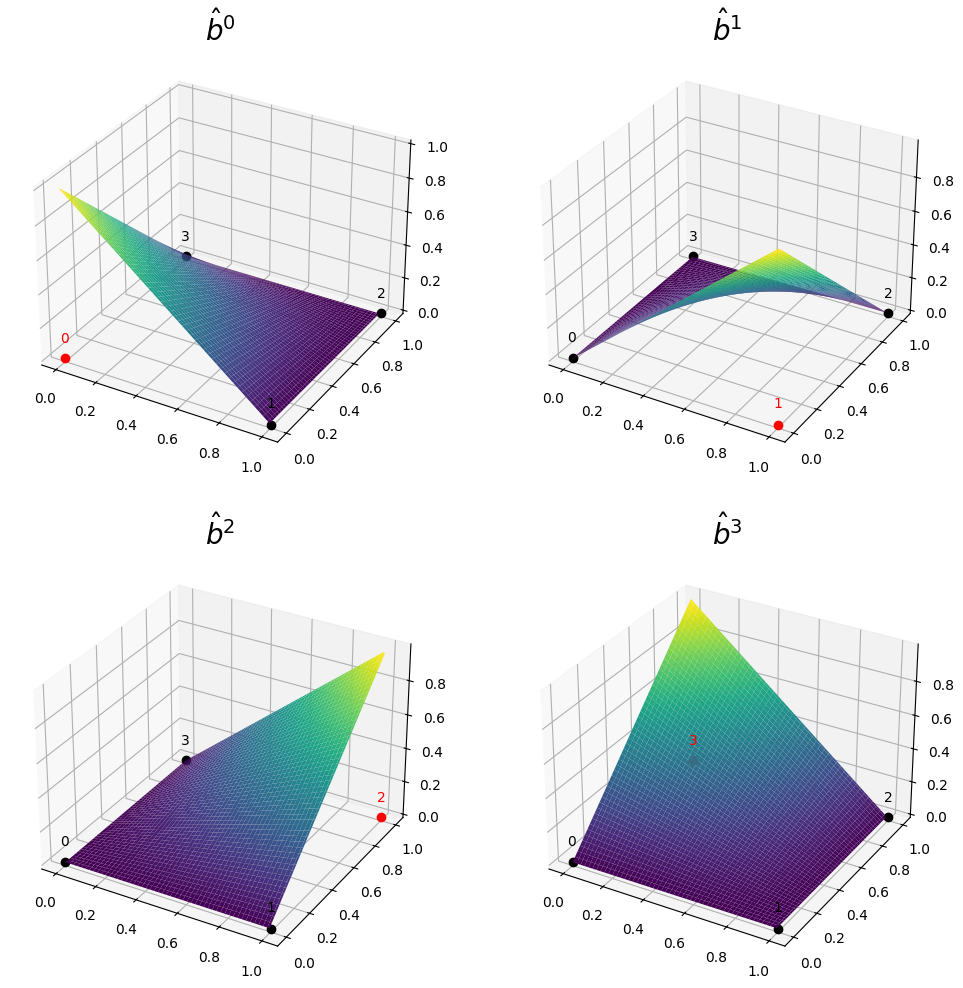
\includegraphics[width=\hsize-2cm]{pictures/lagrange_1st_basis_2d.png}
    \caption{First-order Lagrangian shape functions in 2D.}
    \label{fig:lagrange_1st_2d}
\end{figure}

\subsubsection{Higher-order shape functions}

Higher-order Lagrangian methods have more degrees of freedom per element.
Second-order Lagrangian finite element methods have an additional degree of freedom
in the middle of each edge, in two dimensions also a degree of freedom in the middle of each face
and in three dimensions also an additional degree of freedom in the middle of each cell.

In 1D the shape functions are polynomials of degree two,
specifically, the Lagrangian interpolation polynomials interpolating the points
$0$, $\frac{1}{2}$ and $1$:

\begin{align}
    \label{eq:lagrange_1d_2nd}
    \hat{b}^i(x) = \begin{cases}
                       (1-x)(\frac{1}{2} - x) & i=0, \\
                       x(1-x)                 & i=1, \\
                       x(\frac{1}{2} - x)     & i=2.
                   \end{cases}
\end{align}

\begin{figure}[h]
    \centering
    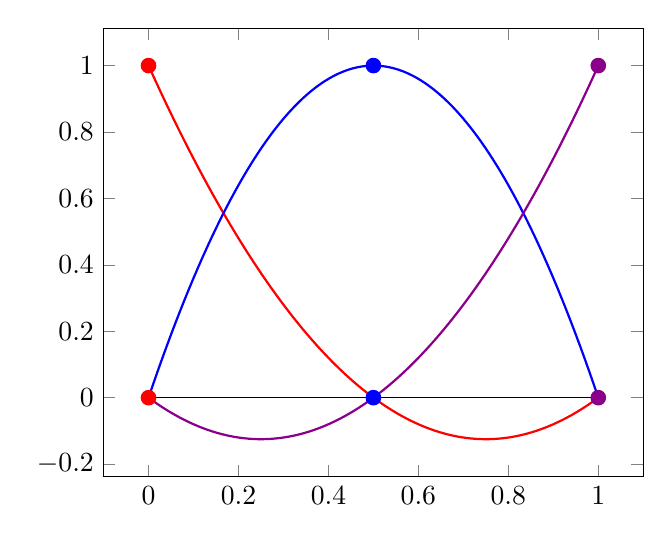
\begin{tikzpicture}
        \begin{axis}[domain=0:1,samples=100]
            \addplot[name path=b0, no markers, color=red, thick] {2 * (x - 0.5) * (x - 1)};
            \addplot[name path=b1, no markers, color=blue, thick] {-4 * x * (x - 1)};
            \addplot[name path=b2, no markers, color=DarkMagenta, thick] {2 * x * (x - 0.5)};
            \addplot[name path=xaxis, black] {0};

            \node[circle, fill=red, inner sep=2pt] at (axis cs:0,0) {};
            \node[circle, fill=red, inner sep=2pt] at (axis cs:0,1) {};

            \node[circle, fill=blue, inner sep=2pt] at (axis cs:0.5,0) {};
            \node[circle, fill=blue, inner sep=2pt] at (axis cs:0.5,1) {};

            \node[circle, fill=DarkMagenta, inner sep=2pt] at (axis cs:1,0) {};
            \node[circle, fill=DarkMagenta, inner sep=2pt] at (axis cs:1,1) {};
        \end{axis}

    \end{tikzpicture}
    \caption{Second-order Lagrange shape functions.}
    \label{fig:2_lagrange_1d}
\end{figure}

The definition for even higher-order Lagrangian finite element spaces and shape functions
follows from the definition of the second-order Lagrangian shape functions (Eq. \ref{eq:lagrange_1d_2nd})
and the interpolating polynomials for more degrees of freedom.

\begin{figure}[h]
    \centering
    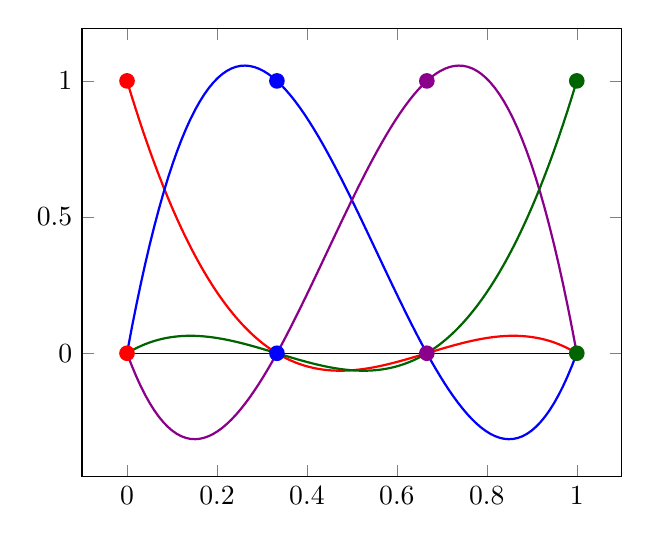
\begin{tikzpicture}
        \begin{axis}[domain=0:1,samples=100]
            \addplot[name path=b0, no markers, color=red, thick] {-(9*x^3) / 2 + 9*x^2 - ((11 * x) / 2) + 1};
            \addplot[name path=b2, no markers, color=blue, thick] {(9 * x * (3 * x^2 - 5 * x + 2)) / 2};
            \addplot[name path=b1, no markers, color=DarkMagenta, thick] {(9*x * (-3*x^2 + 4*x - 1)) / 2};
            \addplot[name path=b3, no markers, color=DarkGreen, thick] {(x * (9 * x^2 - 9 * x + 2)) / 2};
            \addplot[name path=xaxis, black] {0};

            \node[circle, fill=red, inner sep=2pt] at (axis cs:0,0) {};
            \node[circle, fill=red, inner sep=2pt] at (axis cs:0,1) {};

            \node[circle, fill=blue, inner sep=2pt] at (axis cs:1/3,0) {};
            \node[circle, fill=blue, inner sep=2pt] at (axis cs:1/3,1) {};

            \node[circle, fill=DarkMagenta, inner sep=2pt] at (axis cs:2/3,0) {};
            \node[circle, fill=DarkMagenta, inner sep=2pt] at (axis cs:2/3,1) {};

            \node[circle, fill=DarkGreen, inner sep=2pt] at (axis cs:1,0) {};
            \node[circle, fill=DarkGreen, inner sep=2pt] at (axis cs:1,1) {};

        \end{axis}

    \end{tikzpicture}
    \caption{Third-order Lagrange shape functions.}
    \label{fig:3_lagrange_1d}
\end{figure}


\subsection{LagrangeSpace class}
\label{sec:lagrange_class}

The \texttt{LagrangeSpace} class inherits from the \texttt{FiniteElementSpace} class and
overrides and defines the virtual degree of freedom and assembly member functions.

The \texttt{LagrangeSpace} class does not represent the Lagrangian finite element space in a mathematical sense.
It instead serves as a container for all the DOF and assembly operations
corresponding to the rules implied by the Lagrangian finite element space for a specified order.

It takes template arguments for the floating point type \texttt{T}, the dimension \texttt{Dim},
the order \texttt{Order} as well as an argument for the type of the reference element,
the type of the quadrature rule and left-hand-side and right-hand-side field types.

To inherit from the \texttt{FiniteElementSpace} class, it also has to pass a template argument for the
number of element degrees of freedom \texttt{NumElementDOFs}, which is computed at compile
time from the mesh dimension and the order of the \texttt{LagrangeSpace}.


\section{Quadrature}

\label{sec:quadrature}

Numerical quadrature refers to numerical integration in one dimension.

\begin{definition}[$n$-point Quadrature rule]
    An $m$-point quadrature rule on $[a,b]$, $n \in \mathbb{N}$ is defined as \cite{hiptmair_numerical_2023}
    \begin{align}
        \int_a^b f(t) \ \mathrm{d}t \approx \sum_{j=1}^n w_j \, f(x_j),
    \end{align}
    where $w_j \in \R$ are the \emph{quadrature weights} and $x_j \in [a, b]$ are the \emph{quadrature nodes}.
\end{definition}

A quadrature rule defines a way to approximate a definite integral of a function using a weighted sum of the values of the function at specific points, also defined by the quadrature rule, called the quadrature nodes or points.
Quadrature rules have a fixed, total number of points $n$ on which they evaluate the function. For each point $j$ of the $n$ points, the rule also defines a weight for the weighted sum.

In this work, numerical quadrature is required to approximate the integral in the computation of the element matrix of the cell-oriented assembly algorithm (see section \ref{sec:assembly}).

There are many different quadrature rules, with different properties.
To talk about the accuracy of quadrature rules, one can use the \emph{degree of exactness} of a quadrature rule, often abbreviated as just the \emph{degree} of a quadrature rule.

\begin{definition}[Degree of a quadrature rule]
    A quadrature rule has \emph{degree (of exactness)} $m$ if $m$ is the maximal degree of the polynomials
    for which the quadrature rule is guaranteed to be exact \cite[Def.~7.4.1.1]{hiptmair_numerical_2020}.
\end{definition}

This means the quadrature rule of degree $m$ provides exact solutions (instead of just approximations)
for all polynomial functions $f$ with degree lower or equal to $m$. For non-polynomial functions or
polynomials with a degree greater than $m$, it only provides an approximation.

In literature, it is often the order that is used to compare different quadrature rules.

\begin{definition}[Order of a quadrature rule]
    The order $p$ of a quadrature rule of degree $m$ is: \cite[Def.~7.4.1.1]{hiptmair_numerical_2020}
    \begin{align}
        p = m + 1.
    \end{align}
\end{definition}

Some examples of the degrees, and orders, of quadrature rules are:
\begin{itemize}
    \item Midpoint (Rectangle) rule: Degree 1 (Order 2).
    \item Trapezoidal rule: Degree 1 (Order 2).
    \item Simpson rule (3-point): Degree 3 (Order 4).
    \item $n$-point Gaussian quadrature rule: Degree $2n - 1$ (Order $2n$).
\end{itemize}

\subsection{Gaussian-Quadrature}

\begin{definition}[$n$-point Gaussian quadrature rule]
    An $n$-point Gaussian quadrature rule is a quadrature rule that yields exact results for polynomials of degree $2n - 1$ or less.
    It is defined on $[-1, 1]$ as:
    \begin{align}
        \int_{-1}^1 f(x) \ dx \approx \sum_{i=1}^n w_i f(x_i).
    \end{align}
    Therefore, by definition, a Gaussian quadrature rule has degree $2n - 1$ and order $2n$.
\end{definition}

The weights $w_j \in \R, \ j=1, ..., n$ of an $n$-point quadrature rule on $[-1, 1]$ are given by
\cite[Thm.~7.4.1.6]{hiptmair_numerical_2020}:
\begin{align}
    w_j = \int_{-1}^1 L_{j-1}(t) \ dt, \quad j=1, ..., n,
    \label{eq:quad_weights}
\end{align}
where $L_k, \ k = 0, ..., n-1$ is the $k$-th Lagrange polynomial associated with the ordered
set of quadrature nodes $\{ x_1, ..., x_n \}$.

\subsubsection{Gauss-Legendre Quadrature}

The simplest example of a Gaussian quadrature rule is the Gauss-Legendre quadrature rule,
which uses the Legendre polynomials

\begin{definition}[Legendre Polynimial]
    The $n$-th \emph{Legendre polynomial} $P_n$ is defined by \cite[Def.~7.4.2.16]{hiptmair_numerical_2020}:
    \begin{align}
        \int_{-1}^1 P_n(t) q(t) \ dt = 0 \quad \forall q \in \mathcal{P}_{n-1},
    \end{align}
    where $\mathcal{P}_{n-1}$ is the set of polynomials of degree smaller or equal to $n - 1$.

\end{definition}

\begin{definition}[$n$-point Gauss-Legendre Quadrature]
    A $n$-point Gauss-Legendre quadrature rule has the nodes at the zeros (roots) of the $n$-th Legendre polynomial.
    The weights are chosen according to equation \ref{eq:quad_weights}.
\end{definition}


\begin{table}[H]
    \centering
    \renewcommand{\arraystretch}{1.1}
    \small
    \begin{tabularx}{9cm}{>{$}l<{$}| >{$}l<{$}| >{$}l<{$}}
        n & \text{Points} \ x_i         & \text{Weights} \ w_i      \\ \hline
        1 & x_1 = 0                     & w_1 = 2                   \\ \hline
        2 & x_1 = -0.57735026918962...  & w_1 = 1                   \\
          & x_2 = 0.57735026918962...   & w_2 = 1                   \\ \hline
        3 & x_1 = -0.77459666924148...  & w_1 = 0.88888888888888... \\
          & x_2 = 0                     & w_2 = 0.55555555555555... \\
          & x_3 = 0.77459666924148...   & w_3 = 0.88888888888888... \\ \hline
        4 & x_1 = -0.86113631159405...  & w_1 = 0.34785484513745... \\
          & x_2 =  -0.33998104358485... & w_2 = 0.65214515486254... \\
          & x_3 =  0.33998104358485...  & w_3 = 0.65214515486254... \\
          & x_4 =  0.86113631159405...  & w_4 = 0.34785484513745... \\ \hline
        5 & x_1 = -0.90617984593866...  & w_1 = 0.23692688505618... \\
          & x_2 = -0.53846931010568...  & w_2 = 0.47862867049936... \\
          & x_3 = 0                     & w_3 = 0.56888888888888... \\
          & x_4 = 0.53846931010568...   & w_4 = 0.47862867049936... \\
          & x_5 = 0.90617984593866...   & w_5 = 0.23692688505618... \\ \hline
        6 & x_1 = -0.93246951420315...  & w_1 = 0.17132449237917... \\
          & x_2 = -0.66120938646626...  & w_2 = 0.36076157304813... \\
          & x_3 = -0.23861918608319...  & w_3 = 0.46791393457269... \\
          & x_4 = 0.23861918608319...   & w_4 = 0.46791393457269... \\
          & x_5 = 0.66120938646626...   & w_5 = 0.36076157304813... \\
          & x_6 = 0.93246951420315...   & w_6 = 0.17132449237917... \\ \hline
        7 & x_1 = -0.94910791234275...  & w_1 = 0.12948496616887... \\
          & x_2 = -0.74153118559939...  & w_2 = 0.27970539148927... \\
          & x_3 = -0.40584515137739...  & w_3 = 0.38183005050511... \\
          & x_4 = 0                     & w_4 = 0.41795918367346    \\
          & x_5 = 0.40584515137739...   & w_5 = 0.38183005050511... \\
          & x_6 = 0.74153118559939...   & w_6 = 0.27970539148927... \\
          & x_7 = 0.94910791234275...   & w_7 = 0.12948496616887...
    \end{tabularx}
    \caption{Table with Gauss-Legendre quadrature nodes and weights for one to seven points \cite{lowan_table_1942}.}
    \label{table:gauss_legendre}
\end{table}

\pagebreak

\subsection{Gauss-Jacobi Quadrature}

If the function to integrate $f(x), \ f: \R \mapsto [-1, 1]$ has endpoint singularities,
the integrand can be rewritten as $f(x) = (1-x)^\alpha(1+x)^\beta g(x)$,
where $g$ is just the integrable function without the endpoint singularities at $\{-1, 1\}$.
This is known as the Gauss-Jacobi quadrature rule.

\begin{definition}[$n$-point Gauss-Jacobi quadrature rule]
    \begin{align}
        \int_{-1}^1 f(x) \ dx = \int_{-1}^1 (1 - x)^\alpha(1 + x)^\beta g(x) \ dx \approx \sum_{i=1}^n w_i g(x_i),
    \end{align}
    with $\alpha, \ \beta \geq -1$.
\end{definition}

It is important to note that the Gauss-Legendre quadrature is a special case of the Gauss-Jacobi quadrature with $\alpha = \beta = 0$.
Some other special cases of the Gauss-Jacobi quadrature are the Chebyshev-Gauss quadrature of the first kind ($\alpha = \beta = -\frac{1}{2}$),
Chebyshev-Gauss quadrature of the second kind ($\alpha = \beta = \frac{1}{2}$) and Gauss-Gegenbauer quadrature ($\alpha = \beta$).

The Jacobi polynomials, like the Legendre polynomials, are orthogonal polynomials and are defined through a recurrence relation.


\subsubsection*{Algorithm}

To compute the Gauss-Jacobi quadrature nodes, the implementations of deal.II \cite{bangerth_dealiigeneral-purpose_2007},
GSL \cite{gough_gnu_2009}, and LehrFEM++ \cite{craffael_lehrfem_2023} were analyzed.
All of the mentioned libraries use an iterative algorithm to compute the zeros of the polynomials
with the recurrence relation using Newton's method \cite[Chapter~8.5]{hiptmair_numerical_2020}.

The implemented algorithm is mostly based on the implementation from LehrFEM++ \cite{craffael_lehrfem_2023},
since it is best suited our requirements.
For Newton's method, the implementation remained the same as in LehrFEM++.

The steps in the algorithm are:
\begin{enumerate}
    \item Iterate over the number of quadrature points to compute (roots of Gauss-Jacobi polynomial).
    \item For each point, make an initial (educated) guess.
    \item Apply Newton's method on the initial guess to find the root.
    \item Compute the weight corresponding to the point using the root.
\end{enumerate}

The implemented algorithm (see Code \ref{alg:gauss_jac}) also provides the possibility to use different initial guesses.
LehrFEM++ \cite{craffael_lehrfem_2023} uses some custom initial guesses compared to deal.II \cite{bangerth_dealiigeneral-purpose_2007},
which uses the Chebychev nodes for initial guesses.

\begin{Code}
    \small
    \begin{minted}{cpp}
// Compute the root of the Jacobi polynomial
for (std::size_t i = 0; i < NumNodes1D; ++i) {
    // initial guess depending on which root we are computing
    if (initial_guess_type == InitialGuessType::LehrFEM) {
        z = this->getLehrFEMInitialGuess(i, integration_nodes);
    } else if (initial_guess_type == InitialGuessType::Chebyshev) {
        z = -this->getChebyshevNodes(i);
    } else {
        throw std::runtime_error("Unknown initial guess type");
    }

    std::size_t its = 1;
    do {
        // refinement by Newton's method (from LehrFEM++)
        temp = 2.0 + alfbet;

        p1 = (alpha - beta + temp * z) / 2.0;
        p2 = 1.0;
        for (std::size_t j = 2; j <= NumNodes1D; ++j) {
            p3   = p2;
            p2   = p1;
            temp = 2 * j + alfbet;
            a    = 2 * j * (j + alfbet) * (temp - 2.0);
            b    = (temp - 1.0) * (alpha * alpha - beta * beta + temp * (temp - 2.0) * z);
            c    = 2.0 * (j - 1 + alpha) * (j - 1 + beta) * temp;
            p1   = (b * p2 - c * p3) / a;
        }
        pp = (NumNodes1D * (alpha - beta - temp * z) * p1
                + 2.0 * (NumNodes1D + alpha) * (NumNodes1D + beta) * p2)
                / (temp * (1.0 - z * z));

        z1 = z;
        z  = z1 - p1 / pp;  // Newtons Formula

        if (its > this->min_newton_iterations_m && Kokkos::abs(z - z1) <= tolerance) {
            break;
        }
        ++its;
    } while (its <= this->max_newton_iterations_m);

    integration_nodes[i] = z;

    // Compute the weight of the Gauss-Jacobi quadrature
    weights[i] =
        Kokkos::exp(Kokkos::lgamma(alpha + NumNodes1D) + Kokkos::lgamma(beta + NumNodes1D)
                    - Kokkos::lgamma(NumNodes1D + 1.)
                    - Kokkos::lgamma(static_cast<double>(NumNodes1D) + alfbet + 1.0))
        * temp * Kokkos::pow(2.0, alfbet) / (pp * p2);
}
    \end{minted}
    \caption{Abbreviated Algorithm for the computation of the Gauss-Jacobi quadrature nodes and weights.}
    \label{alg:gauss_jac}
\end{Code}


\subsection{Tensor-product Quadrature}

In this chapter, up to now, only one-dimensional quadrature was considered.
However, in this framework, the assembly functions use the quadrature nodes on the reference elements,
which have the same dimension as the mesh that is used.

The reference elements are $n$-cuboids and the quadrature nodes follow the vertices of a tensor-product mesh.

\begin{figure}[h]
    \centering
    \resizebox{0.4\textwidth}{!}{%
        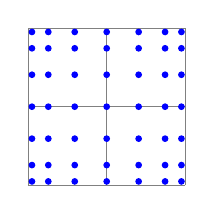
\begin{tikzpicture}
            \draw[step=1cm,gray,very thin] (-1,-1) grid (1,1);
            \foreach \x in {-.94910791234275,-.74153118559939,-.40584515137739,0,.40584515137739,.74153118559939,.94910791234275} {
                    \foreach \y in {-.94910791234275,-.74153118559939,-.40584515137739,0,.40584515137739,.74153118559939,.94910791234275} {
                            \draw[blue,fill=blue] (\x,\y) circle (1pt);
                        }
                }
        \end{tikzpicture}
    }
    \caption{2D Tensor-product of 7-point Gauss-Legendre quadrature nodes on the unit-square.}
    \label{fig:tensor_prod}
\end{figure}


\section{Matrix-free Cell-oriented Assembly Algorithm with Local Computations}

\label{sec:assembly}

Assembly in FEM refers to the computation of the entries of
the stiffness matrix $\mat{A}$ and the entries of the right-hand side vector, or load vector, $\vec{\varphi}$\
of the linear system of equations: $\mat{A}\vec{\mu} = \vec{\varphi}$.

Recall the definition from section \ref{sec:fem_intro} of the stiffness matrix
(Def. \ref{def:stiffness_mat}):

\begin{align}
    \mat{A} = \left[ \mathrm{a}(b_h^j, b_h^i) \right]^N_{i,j=1}, \ \in \R^{N,N},
    \tag{\ref{eq:stiffness_mat}}
\end{align}

and the load vector (Def. \ref{def:load_vec}):

\begin{align}
    \vec{\varphi} = \left[ \ell(b_h^i) \right]^N_{i=1} \in \R^{N}. \tag{\ref{eq:load_vec}}
\end{align}

For each element, we define the \emph{element stiffness matrix} and \emph{element load vector}.

\begin{definition}[Element stiffness matrix and load vector]
    Given a mesh element $K$ and the local shape functions $\{\hat{b}^1, \dots, \hat{b}^M \}$,
    where $M$ is the number of local shape functions, we define the \emph{element stiffness matrix}:
    \begin{align}
        \mat{A}_K := \left[ \mathrm{a}(b_K^j, b_K^i) \right]_{i,j=1}^M \in \R^{M,M},
    \end{align}
    and the \emph{element load vector}:
    \begin{align}
        \vec{\varphi}_K := \left[ \ell(b_K^i) \right]_{i=1}^M \in \R^M.
    \end{align}
\end{definition}

The element stiffness matrix $\mat{A}_K$ has as many rows and columns as there are local degrees of freedom.
For example, for a one-dimensional edge element with the degrees of freedom on the vertices, $\mat{A}_K$ is a
two-by-two matrix. For a 2D mesh and a quadrilateral element with the degrees of freedom also on the vertices,
it is a four-by-four matrix.

The stiffness matrix $\mat{A}$ can be `assembled' by iterating over all the elements,
computing the local element stiffness matrices for every element and then
using them to accumulate the contribution to the global stiffness matrix.
However, in this work, we are using a `matrix-free' assembly algorithm and are
not storing the full global stiffness matrix $\mat{A}$ at any point in time.
The implementation of the matrix-free assembly algorithm is covered in the next section.

\subsection{Matrix-free Assembly Algorithm for the Stiffness Matrix}

As briefly explained in section \ref{sec:matrix_free}, we implemented a
matrix-free assembly algorithm that interfaces with the Conjugate Gradient (CG)
method and returns the product of the stiffness matrix $\mat{A}$ and an
arbitrary vector $\vec{x}$ that is passed to the function: $\mat{A}\vec{x}$.
We call this assembly function \texttt{evaluateAx}
and in addition to the vector $\vec{x}$, it also takes in
a \texttt{C++} Lambda function, named \texttt{eval}, as an input argument.

The \texttt{eval} function evaluates the approximation of the bilinear form
for a given problem. It is defined outside of the assembly function and
passed as an argument to make the assembly function independent of the PDE
that is to be solved.
Later in this section, we derive the assembly function for the Poisson
equation and in the end, we arrive at the assembly function that was implemented
together with the corresponding \texttt{eval} function for the Poisson equation.

The assembly algorithm is cell-oriented, meaning we iterate over all the elements
of the mesh instead of the degrees of freedom. For each element, we perform two
steps. First, we compute the element stiffness matrix $\mat{A}_K$ and second,
we compute the contribution of this element with its corresponding element stiffness matrix,
and the vector $\vec{x}$ to the matrix-vector product $\mat{A}\vec{x}$ that is returned.


Let's start at the first step: Computing the element stiffness matrix $\mat{A}_K$ for a given element $K$.
The entries of the element stiffness matrix are defined using the element bilinear form $\mathrm{a}(\cdot, \cdot)$,
which stems from the weak form of the problem.
The bilinear form of the Poisson equation with homogeneous Dirichlet boundary conditions is (see section \ref{sec:poisson_eq}):
\begin{align}
    (\mat{A}_K)_{i,j} = a(b_K^i, b_K^j) = \int_K \nabla b_K^j \cdot \nabla b_K^i \ d\vec{x}.
\end{align}

However, instead of integrating over a different element $K$ each iteration,
we can transform this integral onto a reference element $\hat{K}$ with unit dimensions
and compute it there ahead of time and then simply do the transformation for every element.

We will briefly explain the variables used in this derivation.
$I$ and $J$ are the global degrees of freedom corresponding to the local degrees of freedom $i$ and $j$.
Where a degree of freedom $I$ corresponds to one or more local degrees of freedom $i$ for different elements if the elements are adjacent
and it lies on the boundaries of those elements.
Given a local degree of freedom $i$, and an element $K$, the choice of the global degree of freedom $I$ is unique.
In the other direction, if a global degree of freedom $I$ is on an element $K$,
the choice of the local degree of freedom for the element is unique as well.
We defined $b_K^I$ and $b_K^J$ to be the shape functions corresponding to the local degrees of freedom $i$ and $j$
of element $K$, defined on the global coordinate system.
The shape functions of the reference element $\hat{K}$ are $\hat{b}_i$ with $i \in {1, ..., M}$, where $M$ is the number
of degrees of freedom on an element.

We start at the definition of the entry of the element stiffness matrix at row $i$ and column $j$,
corresponding to the local degrees of freedom $i$ and $j$ of the element $K$ (Equation \ref{eq:ass_el_stiff_mat_1}).
To compute the integral on the reference element $\hat{K}$ instead of the global element $K$
we use the transformation $\mat{\Phi}_K$ and its pullback $\mat{\Phi}_K^*$ (Equation \ref{eq:ass_el_stiff_mat_2}).
The transformations are defined in section \ref{sec:transformations}.
Next, the pullback is applied to the gradients. This is done to evaluate the gradients of the local shape function on the reference element instead (Equation \ref{eq:ass_el_stiff_mat_3}).
This way, all the computations are done on the reference element and can be precomputed.
After that, we can use numerical quadrature (see section \ref{sec:quadrature}) to approximate the integral (Equation \ref{eq:ass_el_stiff_mat_4}).

\begin{align}
    (\mat{A}_K)_{i,j} & = \int_K \nabla b_K^J(\vec{x}) \cdot \nabla b_K^I(\vec{x}) \ d\vec{x},                                   \label{eq:ass_el_stiff_mat_1} \\
                      & = \int_{\hat{K}} \mat{\Phi}_{K}^* \nabla b_{K}^J(\vec{\hat{x}})
    \cdot \mat{\Phi}_{K}^* \nabla b_{K}^I(\hat{\vec{x}}) \, |\det \mat{D\Phi}_K(\hat{\vec{x}})| \ d\hat{\vec{x}},                \label{eq:ass_el_stiff_mat_2} \\
                      & = \int_{\hat{K}} (\mat{D\Phi}_{K})^{-\top} \nabla \hat{b}^j(\vec{\hat{x}})
    \cdot (\mat{D\Phi}_{K})^{-\top} \nabla \hat{b}^i(\hat{\vec{x}}) |\det \mat{D\Phi}_K(\hat{\vec{x}})| \ d\hat{\vec{x}},        \label{eq:ass_el_stiff_mat_3} \\
                      & \approx \sum_k^{N_\text{Int}} \hat{\omega}_k (\mat{D\Phi}_{K})^{-\top} \nabla \hat{b}^j(\hat{\vec{q}}_k)
    \cdot (\mat{D\Phi}_{K})^{-\top} \nabla \hat{b}^i(\hat{\vec{q}}_k) |\det \mat{D\Phi}_K(\hat{\vec{q}}_k)|,                     \label{eq:ass_el_stiff_mat_4}
\end{align}

where $\hat{\omega}_k$ is the weight of the quadrature rule associated with
$\hat{\vec{q}}_k$, which is the $k$-th quadrature node on the reference element $\hat{K}$.

The eval function is then defined as:
\begin{equation}
    \begin{aligned}
        \texttt{eval}(i, j, k) := (\mat{D \Phi}_K(\hat{\vec{q}}_k))^{-\top}
        \nabla \hat{b}^j(\hat{\vec{q}}_k)
        \cdot
        (\mat{D \Phi}(\hat{\vec{q}}_k))^{-\top}
        \nabla \hat{b}^i(\hat{\vec{q}}_k) \,
        |\det \mat{D \Phi}_K(\hat{\vec{q}}_k)|
    \end{aligned}
    \label{eq:eval}
\end{equation}

The second step in each iteration of the assembly function is the computation of the contribution of the element to the global stiffness matrix $\mat{A}$.
The assembly function returns a vector $\vec{z}$, which is the product of the global stiffness matrix $\mat{A}$ and the vector $\vec{x}$: $\vec{z} = \mat{A}\vec{x}$.
Each entry $\vec{z}_I$ at the global degree of freedom $I$ is the dot-product
of the $I$-th row of $\mat{A}$ and vector $\vec{x}$: $\vec{z}_I = (\mat{A})_{I,:} \cdot \vec{x}$.

Recall that the local degree of freedom $i$ in element $K$ corresponds to a global degree of freedom $I$.
This mapping is stored in the \texttt{FiniteElementSpace} class and is computed once for each element
and then stored at the beginning of each iteration of the assembly algorithm.

The $i$-th entry in the list of global degrees of freedom \texttt{globalDOFs} for element $K$, is the index $I$ of the global degree of freedom.
Therefore the contribution to the global stiffness matrix $\mat{A}$ of an element stiffness matrix $\mat{A}_K$ is computed with:

\begin{algorithm}
    \For{$i\in \texttt{localDOFs}$} {
        $I = \texttt{globalDOFs}[i]$

        \For{$j \in \texttt{localDOFs}$} {
            $J = \texttt{globalDOFs}[j]$

            $(\mat{A})_{I,J} \gets (\mat{A})_{I,J} + (\mat{A}_K)_{i,j}$
        }
    }
\end{algorithm}

To compute the contribution of an element and its corresponding element matrix to the resulting vector $\vec{z}$
we therefore have to add to the $z_I$ entry:

\begin{align}
    \vec{z}_I = \vec{z}_I + (\mat{A}_K)_{i,j} \cdot \vec{x}_J
\end{align}

The pseudocode for the full algorithm for the assembly of the left-hand side (\texttt{evaluateAx}) is given in Algorithm \ref{alg:evalAx}.

\begin{algorithm}[h]
    \vspace{0.5cm}
    \small
    \linespread{1.35}\selectfont
    \KwIn{$\vec{x}$, $\texttt{eval}(i, j, k)$}

    $\vec{z} \gets \vec{0}$ {\color{darkgray}\tcp{Resulting vector to return}}

    \For{Element $K$ in Mesh}{

    $\texttt{localDOFs} \gets \texttt{getLocalDOFsForElement}(K)$

    $\texttt{globalDOFs} \gets \texttt{getGlobalDOFsForElement}(K)$

    {\color{darkgray}\tcp{1. Compute the Element matrix $\mat{A}_K$}}

    \For{$i \in \texttt{localDOFs}$}{
    \For{$j \in \texttt{localDOFs}$}{
    $\displaystyle
        (\mat{A}_K)_{i,j} \approx \sum_{k}^{N_\text{Int}}
        \hat{\omega}_k
        \underbrace{
            (\mat{D \Phi}_K(\hat{\vec{q}}_k))^{-\top}
            \nabla \hat{b}^j(\hat{\vec{q}}_k)
            \cdot
            (\mat{D \Phi}(\hat{\vec{q}}_k))^{-\top}
            \nabla \hat{b}^i(\hat{\vec{q}}_k) \,
            |\det \mat{D \Phi}_K(\hat{\vec{q}}_k)|
        }_{=:\texttt{eval}(i, j, k)}
    $
    }}

    {\color{darkgray}\tcp{2. Compute $\vec{z} = \mat{A}\vec{x}$ contribution with $\mat{A}_K$}}
    \For{$i\in \texttt{localDOFs}$} {
        $I = \texttt{globalDOFs}[i]$

        \For{$j \in \texttt{localDOFs}$} {
            $J = \texttt{globalDOFs}[j]$

            $\vec{z}_I \gets \vec{z}_I + (\mat{A}_K)_{i,j} \cdot \vec{x}_J$
        }
    }
    }
    \KwRet{$\vec{z}$}
    \vspace{0.5cm}

    \caption{\texttt{evaluateAx} (for the specific case of the Poisson equation).}
    \label{alg:evalAx}
\end{algorithm}

\subsection{Assembly Algorithm for the Load Vector}

The assembly algorithm for the right-hand-side is very similar to the left-hand side:
\begin{enumerate}
    \item Assembly of the element load vector.
    \item Accumulation of the contribution to $\vec{\varphi}$.
\end{enumerate}

The linear form of the load vector is (from section \ref{sec:fem_intro}):
\begin{align}
    \ell(b^I_K) = \int_K f(\vec{x}) b^I_K(\vec{x}) \ d\vec{x},
\end{align}

where $f$ is the source function and $b^I_K$ is the shape function of the $I$-th global degree of freedom of element $K$.

Using the method outlined in the previous section, we arrive at the algorithm for the computation of the
load vector shown in Algorithm \ref{alg:evalLoadVector}.
For this assembly function of the right-hand side, we don't pass an \texttt{eval} function
but the right-hand side source function $f$.

\begin{algorithm}[h]
    \vspace{0.5cm}
    \small
    \linespread{1.35}\selectfont
    \KwIn{$\vec{x}$, $f$}

    $\vec{\varphi} \gets \vec{0}$ {\color{darkgray}\tcp{Resulting load vector to return}}

    \For{Element $K$ in Mesh}{

    $\texttt{localDOFs} \gets \texttt{getLocalDOFsForElement}(K)$

    $\texttt{globalDOFs} \gets \texttt{getGlobalDOFsForElement}(K)$

    {\color{darkgray}\tcp{1. Compute the Element matrix $\mat{A}_K$}}

    \For{$i \in \texttt{localDOFs}$}{
    $\displaystyle
        (\vec{\varphi}_K)_{i} \approx \sum_{k}^{N_\text{Int}}
        \hat{\omega}_k
        f(\mat{\Phi}_K(\hat{\vec{x}})) \hat{b}^i(\hat{\vec{q}}_k) \,
        |\det \mat{D \Phi}_K(\hat{\vec{q}}_k)|
    $
    }

    {\color{darkgray}\tcp{2. Compute load vector $\vec{\varphi}$ contribution of $\vec{\varphi}_K$}}
    \For{$i\in \texttt{localDOFs}$} {
        $I = \texttt{globalDOFs}[i]$

        $\vec{\varphi}_I \gets \vec{\varphi}_I + (\vec{\varphi}_K)_i$
    }
    }
    \KwRet{$\vec{\varphi}$}
    \vspace{0.5cm}
    \caption{\texttt{evaluateLoadVector} (for the specific case of the Poisson equation).}
    \label{alg:evalLoadVector}
\end{algorithm}

\subsection{Essential Boundary conditions}

In FEM, Dirichlet boundary conditions are synonymous with essential boundary conditions.

Essential boundary conditions are enforced on the functions in the trial space.
Natural boundary conditions or Neumann boundary conditions, are enforced through the variational equation.
They therefore appear in the bilinear form and are implemented in the \texttt{eval} function of the problem.


\subsubsection{Homogeneous Dirichlet Boundary Conditions}

To implement homogeneous Dirichlet boundary conditions, or zero Dirichlet boundary conditions,
one can set the entries of the stiffness matrix corresponding to the degrees of freedom on the boundary to zero
\cite[Chapter~2.7.6]{hiptmair_numerical_2023}.

To support them, the left-hand-side assembly algorithm was modified to skip all DOFs on the boundary when accumulating the contributions
from the element stiffness matrices to force them to be zero.

Due to time constraints, we must leave heterogeneous Dirichlet boundary conditions,
and other types of boundary conditions, to be implemented in future work.

\section{Solver}
\label{sec:solver}

The \texttt{FEMPoissonSolver} class inherits from the IPPL \texttt{Poisson} class and follows in functionality
the existing IPPL \texttt{PoissonCG} class.
This new solver class provides a constructor, a solve function and getters for the total number
of iterations and the residue after solving.
The constructor takes in a left-hand-side IPPL \texttt{Field}, a right-hand-side IPPL \texttt{Field} and the source function $f$.
In the constructor, the right-hand-side field values are then set according to the
\texttt{evaluateLoadVector} assembly function with the given source function $f$.

Inside the \texttt{solve} function, the \texttt{eval} lambda function for the Poisson equation is defined.
The \texttt{eval} function is a function that depends on the PDE weak form and is used to decouple the
assembly function from the problem itself. It is passed to the assembly function which
provides the arguments needed to solve the problem.

For the Poisson equation, the \texttt{eval} function is:
\begin{align}
    \text{eval}(i, j, k) = (\mat{D \Phi}_K^{-\top}) \nabla \hat{b}^j(\vec{q}_k) \cdot
    (\mat{D \Phi}_K^{-\top}) \nabla \hat{b}^i(\vec{q}_k)
    |\det \mat{D \Phi}_K|,
\end{align}
where $i$ and $j$ are the indices for the local degrees of freedom used
to select the corresponding reference element shape function and
$\vec{q}_k$ is the $k$-th integration point.

It is important to note, that everything in this \texttt{eval} function can be pre-computed because
everything is evaluated on the reference element (see section \ref{sec:elements}).

Inside the \texttt{FEMPoissonSolver}, the transformation variables $\mat{D \Phi}^{-\top}$
and $|\det \mat{D \Phi}|$ are pre-computed but the values of the basis functions
at the quadrature nodes $k$ are precomputed inside the assembly function instead
and passed by reference to the \texttt{eval} function.
In the future, the signature of the \texttt{eval} function might need tweaking to support
problems that have more than the gradient of the basis in their weak form.

\begin{Code}
    \begin{minted}{cpp}
const auto poissonEquationEval =
    [DPhiInvT, absDetDPhi](
        const std::size_t& i, const std::size_t& j,
        const Vector<Vector<Tlhs, Dim>, NumElementDOFs>& grad_b_q_k) {
        return dot((DPhiInvT * grad_b_q_k[j]), (DPhiInvT * grad_b_q_k[i])).apply()
                * absDetDPhi;
    };
\end{minted}
    \caption{\texttt{eval} function implementation from \texttt{FEMPoissonSolver}.}
\end{Code}

In the \texttt{FEMPoissonSolver}, after pre-computation of the transformation variables,
the IPPL \texttt{PCG} (Preconditioned Conjugate Gradient) algorithm class is used
to solve the linear system of equations.

Currently, the \texttt{FEMPoissonSolver} is using Gauss-Legendre quadrature with five integration points in one dimension.
It is used by initializing the
\texttt{GaussJacobiQuadrature} class with the parameters $\alpha = \beta = 0$.
points and first-order Lagrangian Finite Elements using the \texttt{LagrangeSpace} class.

The dimension of the mesh is the same as the dimension of the input fields that are passed to the constructor.


\section{Results}

Using the \texttt{FEMPoissonSolver}, outlined in the previous section (see section \ref{sec:solver}),
we computed the solutions for a given problem and studied the convergence to the
exact solution for decreasing mesh spacings (mesh refinement).
The accuracy was tested for one, two and three dimensions and the convergence was good for each of them.

The problem solved was the Poisson equation with a sinusoidal source function
and homogenous Dirichlet boundary conditions.
In one dimension, the problem was:
\begin{align}
    -\Delta u = \pi^2 \sin(\pi x), \quad x \in [-1, 1],
\end{align}
with $u(-1) = 0$ and $u(1) = 0$.
The exact solution to this problem is:
\begin{align}
    u(x) = \sin(\pi x).
\end{align}

To solve this problem in two and three dimensions, the following $N$-dimensional variant of the same problem was used:
\begin{align}
    -\Delta u = N \pi^2 \prod_{i=1}^N \sin(\pi \vec{x}_i), \quad \vec{x} \in [-1, 1]^N,
\end{align}
where $N \in \mathbb{N}$ is the number of dimensions, the solution function $u$ is defined as:
$u: \R^N \to \R$, with the $N$-dimensional point $\vec{x} \in \R^N$ with its elements $\vec{x}_i \in \R : \ \vec{x}_i \in \vec{x}$ with $i \in \{1, ..., N\}$.
Also, the function $u$ is zero on the boundaries: $u(\vec{x}) = 0$ if for any entry $\vec{x}_i \in \vec{x}$,
it holds that $\vec{x}_i \in \{-1, 1\}$ for $i \in \{1, ..., N\}$.

This problem has the exact solution:

\begin{align}
    u(\vec{x}) = \prod_{i=1}^N \sin(\pi \vec{x}_i).
\end{align}

This test along with these sinusoidal functions are implemented in \texttt{TestFEMPoissonSolver}.

Different numbers of mesh vertices of powers of two were used in each dimension.
For a given number of mesh vertices $n$, the mesh spacing $h$ is given by:
\begin{align}
    h = \frac{2}{n - 1}.
    \label{eq:spacing}
\end{align}

The tolerance used in the CG algorithm was chosen to be $10^{-13}$.

In table \ref{table:sinusoidal_1d} the number of mesh vertices $n$ is given in the `Size column',
the `Spacing' is computed via equation \ref{eq:spacing}, the `Relative Error' is the relative error
of the computed solution compared to the analytical solution of the problem, the `Residue' is the
residue from the CG algorithm (see Algorithm \ref{alg:conjugate_gradient}) and the number of iterations
of the CG algorithm is given in the `Iterations' column.

\begin{table}[H]
    \centering
    \renewcommand{\arraystretch}{1.1}
    \small
    \begin{tabularx}{\hsize}{l l l l l}
        Size & Spacing              & Relative Error        & Residue               & Iterations \\ \hline
        4    & 0.6666666666666666   & 7.080989919320194e-09 & 4.440892098500626e-16 & 1          \\
        8    & 0.2857142857142857   & 1.249845927172312e-12 & 2.094764613337708e-15 & 1          \\
        16   & 0.1333333333333333   & 6.407420160623263e-16 & 5.325889242270741e-15 & 1          \\
        32   & 0.06451612903225806  & 1.779759178867111e-15 & 1.742186992884441e-14 & 1          \\
        64   & 0.03174603174603174  & 1.789223255831461e-16 & 6.654398136858673e-14 & 1          \\
        128  & 0.01574803149606299  & 3.503924460135148e-15 & 5.157582646417248e-14 & 2          \\
        256  & 0.007843137254901961 & 7.471370361275646e-15 & 8.253791443434346e-14 & 3          \\
        512  & 0.003913894324853229 & 2.094557289636767e-15 & 4.997105441592253e-14 & 5          \\
        1024 & 0.001955034213098729 & 2.178897100917102e-14 & 4.308783938700041e-14 & 177
    \end{tabularx}
    \caption{\texttt{TestFEMPoissonSolver} Output for the 1D sinusoidal problem.}
    \label{table:sinusoidal_1d}
\end{table}

\begin{figure}[H]
    \centering
    \includegraphics[width=12cm]{pictures/fem_convergence_sinus1d.png}
    \caption{1D Sinusoidal convergence}
    \label{fig:convergence_sinusoidal_1d}
\end{figure}

For one dimension, the solution converges with order 10 until it gets close to machine precision
(figure \ref{fig:convergence_sinusoidal_1d}).
This is much faster than anticipated and we assume it is
due to the smooth, periodic nature of the right-hand side chosen.
At the moment the solver only uses first-order Lagrangian finite element methods,
which are linear functions (see figure \ref{fig:1_lagrange_1d}).
There is a phenomenon for the trapezoidal quadrature rule, where it converges rapidly
when applied to analytic functions on periodic intervals \cite{trefethen_exponentially_2014}.

We think the convergence we are seeing for one dimension might be related to this phenomenon,
however, this was not investigated further but it might be interesting for future work.

\begin{table}[H]
    \centering
    \renewcommand{\arraystretch}{1.1}
    \small
    \begin{tabularx}{\hsize}{l l l l l}
        Size & Spacing              & Relative Error        & Residue               & Iterations \\ \hline
        4    & 0.6666666666666666   & 0.367835959800294     & 8.881784197001252e-16 & 1          \\
        8    & 0.2857142857142857   & 0.06877172889870629   & 2.054662609310059e-15 & 1          \\
        16   & 0.1333333333333333   & 0.01470558224055019   & 6.673718396468935e-15 & 1          \\
        32   & 0.06451612903225806  & 0.003428048120959612  & 1.226637297968919e-14 & 1          \\
        64   & 0.03174603174603174  & 0.0008291654851627174 & 2.735745689195284e-14 & 1          \\
        128  & 0.01574803149606299  & 0.0002039888701591884 & 1.157673913473065e-14 & 2          \\
        256  & 0.007843137254901961 & 5.059492109621404e-05 & 1.26186832683033e-14  & 3          \\
        512  & 0.003913894324853229 & 1.259908312652751e-05 & 7.423183529194849e-15 & 119        \\
        1024 & 0.001955034213098729 & 3.143610123038628e-06 & 3.751402450611288e-15 & 265
    \end{tabularx}
    \caption{\texttt{TestFEMPoissonSolver} Output for the 2D sinusoidal problem.}
    \label{table:convergence_sinusoidal_2d}
\end{table}


\begin{figure}[H]
    \centering
    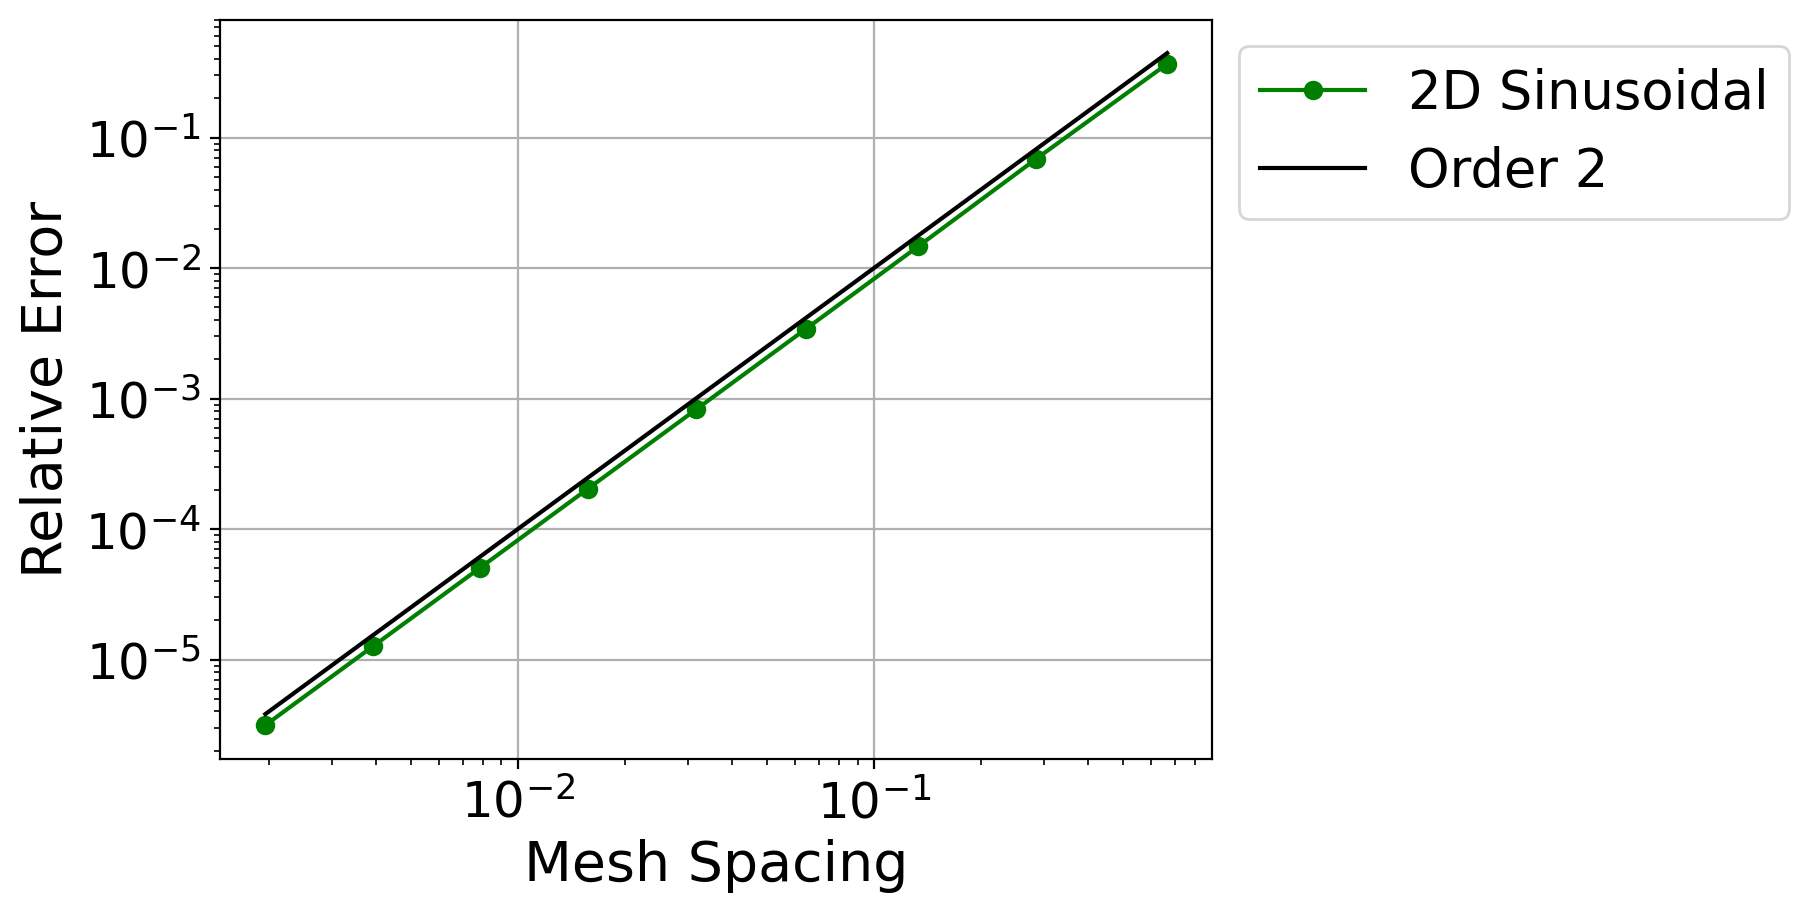
\includegraphics[width=12cm]{pictures/fem_convergence_sinus2d.png}
    \caption{2D Sinusoidal convergence}
    \label{fig:convergence_sinusoidal_2d}
\end{figure}

In two dimensions, the fast convergence from the one-dimensional study disappears and
it follows second-order convergence. This is the minimal rate of convergence expected for FEM
but it is to be expected for first-order Lagrangian finite elements.

\begin{table}[H]
    \centering
    \renewcommand{\arraystretch}{1.1}
    \small
    \begin{tabularx}{\hsize}{l l l l l}
        Size & Spacing             & Relative Error        & Residue               & Iterations \\ \hline
        4    & 0.6666666666666666  & 0.8709752261711512    & 1.368774871883577e-15 & 1          \\
        8    & 0.2857142857142857  & 0.1422730084945544    & 8.763930132546234e-15 & 1          \\
        16   & 0.1333333333333333  & 0.02962741863012481   & 1.814959731383155e-14 & 1          \\
        32   & 0.06451612903225806 & 0.006867847755836543  & 1.019648580795529e-14 & 1          \\
        64   & 0.03174603174603174 & 0.00165901848558236   & 1.623920791356438e-14 & 1          \\
        128  & 0.01574803149606299 & 0.0004080193515153442 & 3.485107117806992e-15 & 10
    \end{tabularx}
    \caption{\texttt{TestFEMPoissonSolver} Output for the 3D sinusoidal problem.}
    \label{table:sinusoidal_3d}
\end{table}


\begin{figure}[H]
    \centering
    \includegraphics[width=12cm]{pictures/fem_convergence_sinus3d.png}
    \caption{3D Sinusoidal convergence}
    \label{fig:convergence_sinusoidal_3d}
\end{figure}


In three dimensions, we get a very similar picture as in two dimensions.
We also observe second-order convergence.

Note: For three dimensions, the relative error was not computed for more than 128 mesh vertices (in each dimension)
due to the high computational load and the serial nature of this implementation.


\chapter{Conclusion}

This thesis and the implemented building blocks for it are the first big step into FEM
for IPPL. It not only contains the building blocks for FEM, it can already be considered a FEM
framework by itself, with the inclusion of the solver.
We have shown the implementation from the ground up and have been able to achieve good
convergence using the solver.

% Design
% Elements
% Finite Element Space
% LagrangeSpace and basis functions
% Quadrature
% Assembly
% Solver

We started by designing the general software architecture of the \texttt{C++} FEM framework in IPPL,
with extensibility in mind.
Then, element classes along with dimension-independent affine transformations were implemented,
followed by the \texttt{FiniteElementSpace} base class handling the mapping of the mesh to the elements.
Then the \texttt{LagrangeSpace} class was implemented, which supports first-order Lagrangian finite elements,
for one- to three-dimensional meshes. It was also designed to be easily extensible to higher-order basis functions.
Next, a base class for numerical quadrature was added which has methods for creating
tensor-product quadrature points and weights for all the reference elements. It serves
as the basis of the Midpoint quadrature rule and the Gauss-Jacobi quadrature rule which were also implemented
in this work.
The latter uses an iterative algorithm to compute the roots of the Jacobi-Polynomial.
With the main building blocks taken care of, a special matrix-free assembly algorithm, interfacing with the CG method,
was implemented for ideal performance on GPUs, in the future.
And finally, the \texttt{FEMPoissonSolver} was added as a proof-of-concept and as an example
for future FEM solvers.



\section{Future Work}
\label{sec:future_work}

This thesis is still only the beginning for FEM in IPPL.
In future work, one could continue with higher-order Lagrangian finite elements,
adding support for more boundary conditions
(i.e non-homogeneous Dirichlet boundary conditions or periodic boundary conditions) and
process- and thread-level parallelization.
Then it would be interesting to do some timing studies and GPU benchmarks.
After that, more \texttt{FinitElementSpace} classes could be implemented
(i.e. Nédélec or Raviart-Thomas finite elements), on the road to solving the electromagnetic Maxwell equations.

We provide some guidance and our thoughts on the implementation
of some of these topics in Appendix \ref{chp:implementation_help}.

\section*{Acknowledgements}

I would like to thank the AMAS group from PSI and Dr. Andreas Adelmann for their support
and their trust to let me begin the work of implementing FEM in the IPPL framework.
I especially want to thank my scientific advisor Ms. Sonali Mayani who supported me greatly
throughout this thesis, it was great working with her.


\bibliography{thesis.bib}

\begin{appendices}
    

\chapter{Resources and Details}

\section{Resources}

\begin{itemize}
    \item IPPL repository (GitHub): \href{https://github.com/IPPL-framework/ippl}{https://github.com/IPPL-framework/ippl}
    \item IPPL FEM branch (GitHub): \href{https://github.com/s-mayani/ippl/tree/fem-framework}{https://github.com/s-mayani/ippl/tree/fem-framework}
    \item IPPL build scripts (GitHub): \href{https://github.com/IPPL-framework/ippl-build-scripts}{https://github.com/IPPL-framework/ippl-build-scripts}
    \item Student repository (PSI GitLab): \href{https://gitlab.psi.ch/AMAS-students/buehler\_bsc}{https://gitlab.psi.ch/AMAS-students/buehler\_bsc}
\end{itemize}

\section{IPPL Build Instructions}

\begin{enumerate}
    \item Make sure the following prerequisites are installed:

          \begin{itemize}
              \item curl (\href{https://curl.se}{https://curl.se})
              \item git (\href{https://git-scm.com}{https://git-scm.com})
              \item Make (\href{https://www.gnu.org/software/make}{https://www.gnu.org/software/make})
              \item CMake (\href{https://cmake.org}{https://cmake.org})
              \item A compatible C++ compiler:
                    \begin{itemize}
                        \item GCC (\href{https://gcc.gnu.org}{https://gcc.gnu.org})
                        \item Clang (\href{https://clang.llvm.org}{https://clang.llvm.org})
                    \end{itemize}
              \item MPI, for example OpenMPI (\href{https://www.open-mpi.org}{https://www.open-mpi.org})
              \item GoogleTest (\href{https://github.com/google/googletest}{https://github.com/google/googletest})
          \end{itemize}

    \item Clone the build script repository.

          \texttt{git clone https://github.com/IPPL-framework/ippl-build-scripts.git}

          This will clone four Bash scripts into a new \texttt{ippl-build-scripts} directory:

          \begin{itemize}
              \item \texttt{100-build-kokkos}
              \item \texttt{200-build-heffte}
              \item \texttt{300-build-ippl}
              \item \texttt{999-build-everything}
          \end{itemize}

          The scripts are used to set up all the dependencies, as well as for building IPPL itself.

          The commit used at the time of writing of the \texttt{ippl-build-scripts} repository was commit \texttt{e9a3e1f},
          in later commits, some steps might be different.

          To switch to that commit, run: \texttt{git checkout e9a3e1f}

    \item Set up the build scripts to use the FEM branch.

          The IPPL FEM framework was developed in a separate fork of the IPPL repository (listed as ``IPPL FEM branch'' in the `Resources' section).
          At the time of writing, the FEM framework introduced in this thesis was not yet merged
          into any branch of the official IPPL GitHub repository, but instead lives in a branch in the forked repository.
          If the FEM framework was merged into the \texttt{main} branch in the meantime, this step can be safely ignored.
          If it was not yet merged, the URL of the IPPL repository needs to be altered in the \texttt{300-build-ippl} Bash script and the branch needs to be switched.

          The unaltered script (\texttt{300-build-ippl}) contains the following snippet given in Code \ref{code:script-ippl-1}.

          \begin{Code}
              \begin{minted}{sh}
        if [ -d "ippl" ] 
        then
            echo "Found existing IPPL source directory"
        else
            echo "Clone ippl repo ... "
            if [ ! -z "$USE_SSH" ]; then
                git clone git@github.com:IPPL-framework/ippl.git
            else
                git clone https://github.com/IPPL-framework/ippl.git
            fi
        fi
          \end{minted}
              \caption{Unaltered script snippet from \texttt{300-build-ippl}}
              \label{code:script-ippl-1}
          \end{Code}

          In this snippet, we need to alter the repository URL to the URL of the repository that contains
          the FEM framework. Additionally, we add \texttt{git} commands to switch the branch after cloning.

          The script should be altered to make the above snippet look like the following snippet given in Code \ref{code:script-ippl-2}.

          \begin{Code}
              \begin{minted}{bash}
        if [ -d "ippl" ] 
        then
            echo "Found existing IPPL source directory"
        else
            echo "Clone ippl repo ... "
            if [ ! -z "$USE_SSH" ]; then
                git clone git@github.com:s-mayani/ippl.git ippl
            else
                git clone https://github.com/s-mayani/ippl.git ippl
            fi
            # Navigate into the cloned folder to switch the branch
            cd ippl
            git fetch
            git switch fem-framework
            cd ..
        fi
          \end{minted}
              \caption{Altered script snippet from \texttt{300-build-ippl}}
              \label{code:script-ippl-2}
          \end{Code}

          After altering the script, it will now clone the desired repository and switch to the FEM branch.

    \item Run the build scripts to install the dependencies and build ippl.

          All that is left to do is run the build scripts with the desired options to build the IPPL repository.
          The available options can be found in the \texttt{README} of the build scripts repository under ``Flags''.

          To build everything, run the following command:

          \texttt{./999-build-everything -t serial -kfi --export}

          The command will also set the required environment variables.
          The \texttt{-t} argument sets the build target, \texttt{-k} installs Kokkos,
          \texttt{-f} installs heFFTe and \texttt{-i} installs IPPL.

          Running the command from above, will create a directory for ippl and inside it
          a build directory \texttt{ippl-build-scripts/ippl/build\_serial/}.
          This build directory will contain all the executables.
          To rebuild in the future, navigate inside this directory and use \texttt{make}.

\end{enumerate}

\section{Documentation Build Instructions}
\label{app:doxygen}

The IPPL framework has a Doxygen documentation that can be built locally,
and viewed in the browser.
To build it, make sure you have Doxygen and its prerequisites installed.
Then navigate into the \texttt{doc/} directory in the IPPL repository
and run the following command:

\begin{minted}{bash}
doxygen Doxyfile
\end{minted}

Then simply open the file \texttt{doc/html/index.html} in the browser of your choice to read the
documentation.

\pagebreak

\section{Plot Generation}

Each of the plots used in this work is produced in two steps.
In the first step, the data is generated by running a test executable, which is compiled when building IPPL,
and the generated data is stored in a file. This will be either a Comma-Separated Values (CSV) file
or a text file that stores the raw output.
In the second step, the data is plotted using Python and a Jupyter Notebook.

The Jupyter Notebooks can be found in the student repository (PSI GitLab) inside the plots directory.
Inside the \texttt{plots} directory, there are two directories,
\texttt{convergence} containing the convergences plots and the corresponding Jupyter notebook
and \texttt{lagrange\_space} containing two directories for 1D and 2D.

\subsection{Lagrangian finite element space plots}

For the \texttt{LagrangeSpace} plots, the executables are inside the build directory
(\texttt{build\_serial}, \texttt{build\_openmp}, etc.), under \texttt{<build\_dir>/test/FEM/}.
Where an executable for 1D and one for 2D can be found: \texttt{TestLagrangeSpace1D} and \texttt{TestLagrangeSpace2D}.
Their source files can be found under \texttt{src/test/FEM/}.

After running the executables and before running the notebooks, copy the generated CSV files \texttt{1D\_lagrange\_local\_basis.csv} and
\texttt{2D\_lagrange\_local\_basis.csv} to the same directory as the notebooks named

To create the plot for 1D, run the Jupyter notebook named \texttt{plot\_lagrange\_1d.ipynb} at \texttt{plots/lagrange\_space/1d}
in the student GitLab repository
and for 2D run the Jupyter Notebook \texttt{plot\_lagrange\_2d.ipynb} at \texttt{plots/lagrange\_space/2d}.

This will generate the plot from figure \ref{fig:lagrange_1st_2d}.

\subsection{Convergence plots}

For the FEM convergence plot, the test is located in the \texttt{solver} directory in the build folder.
The test is called \texttt{TestFEMPoissonSolver}. (\texttt{<build\_dir>/solver/TestFEMPoissonSolver}).
The source file for this test is located at \texttt{/src/test/solver/TestFEMPoissonSolver.cpp}.
Run the executables and store the output in a text file. I chose the naming scheme of \texttt{sinus1d.dat} to \texttt{sinus3d.dat}
depending on the number of dimensions.

Run the executable from the build directory with the command below,
by replacing \texttt{<Dim>} with the integer 1, 2, or 3 for 1D, 2D and 3D:
\begin{minted}{sh}
./test/solver/TestFEMPoissonSolver <Dim> --info 5 > sinus<Dim>d.dat
\end{minted}

The output will be piped into a file called \texttt{sinus1d.dat}, \texttt{sinus2d.dat} or \texttt{sinus3d.dat} in the build directory.
After running the solver test for all three dimensions,
copy all three files for the three dimensions to \texttt{plots/convergence} in the student GitLab repository.
Then simply run the Jupyter Notebook in the same directory called \texttt{convergence.ipynb}.

This will generate the plots from figures \ref{fig:convergence_sinusoidal_1d}, \ref{fig:convergence_sinusoidal_2d} and \ref{fig:convergence_sinusoidal_3d}.


    \chapter{Implementation Helpers}

\label{chp:implementation_help}

The purpose of this section is to give some guidance and thoughts on the implementation
of some of the topics mentioned in the Future Work section (section \ref{sec:future_work}).
Since we have not implemented the problems described in this section, we
are not able to provide all the details for the respective implementations at this time,
but we can provide some pointers as to where the current implementation needs to change
and provide some additional thoughts where applicable.

\section{Higher-order Lagrangian finite elements}

Something we planned on implementing, but ran out of time for, were higher-order Lagrangian finite elements.
The implementation in the \texttt{LagrangeSpace} class will need to be updated as well as the corresponding unit tests.
The \texttt{LagrangeSpace} class already has a template argument for the order that is used in some functions and unit tests.
In the \texttt{LagrangeSpace} class both the DOF functions need to be updated,
as well as the functions that evaluate the shape function and the gradient of the shape function on the
reference element at a given point on the reference element.



\section{Non-homogeneous Dirichlet boundary conditions}

For non-homogeneous Dirichlet boundary conditions, the assembly function
\texttt{evaluateAx} in the \texttt{LagrangeSpace} needs to be updated, as well as the corresponding unit tests.
The first change should be making the assembly function know which boundary condition it is dealing with.
The type of boundary condition is stored in the field and should be retrieved from the LHS field object.

Currently, in the assembly function, it assumes homogeneous Dirichlet boundary conditions.
Under this assumption, the current implementation skips all the DOFs on the boundary
when accumulating the contribution to the resulting vector $\vec{z}$.
This is done to set the assembly matrix to zero for degrees of freedom on the boundary.
This behavior will need to be modified to implement the non-homogeneous Dirichlet boundary conditions.
Please refer to \cite[Chapter~2.7.6]{hiptmair_numerical_2023} for more details on how to implement them.

\section{Other Finite Elements and their spaces}

An essential step in implementing the electromagnetic solver with the Finite Element Time Domain (FETD)
scheme is the implementation of the Nédélec and Raviart-Thomas finite element methods.

To add a new finite element type, one needs to implement a new class that inherits from the \texttt{FiniteElementSpace} class
and implements all the pure virtual functions from it.
Meaning, that all the functions needed for the mapping from the local DOFs to the global DOFs and vice-versa need to be implemented,
as well as the functions that evaluate the shape function and its gradient on the reference element.
These functions should be implemented to be dimension-independent if possible, or at least work for 1D, 2D and 3D.
As the next step, these implementations should also work for higher-order elements of the new type.

The functions that need to be implemented are:

\vspace*{0.5cm}\noindent
\begin{tabular}{| l | p{6.5cm} |}
    \hline
    \texttt{numGlobalDOFs}                           & Returns the number of global degrees of freedom (DOFs) in the space for a given mesh.                                                            \\ \hline
    \texttt{getLocalDOFIndex}                        & Returns the local DOF for a given element and a given global DOF.                                                                                \\ \hline
    \texttt{getGlobalDOFIndex}                       & Returns the global DOF given an element and a local DOF.                                                                                         \\ \hline
    \texttt{getLocalDOFIndices}                      & Returns the vector of local DOFs for the reference element for this space.                                                                       \\ \hline
    \texttt{getGlobalDOFIndices}                     & Returns the global DOFs for a given element.                                                                                                     \\ \hline
    \texttt{getGlobalDOFNDIndices}                   & Returns a vector of \texttt{NDIndex} for the global DOFs of a given element.                                                                     \\ \hline
    \texttt{evaluateRefElementShapeFunction}         & Returns the scalar value of the reference element shape function for the given local DOF and given point on the reference element.               \\ \hline
    \texttt{evaluateRefElementShapeFunctionGradient} & Returns the scalar value of the gradient of the reference element shape function for a given local DOF and local point on the reference element. \\ \hline
    \texttt{evaluateAx}                              & This is the assembly function for the left-hand side. For reference refer to the implementation in \texttt{LagrangeSpace}.                       \\ \hline
    \texttt{evaluateLoadVector}                      & This is the assembly function for the right-hand side. For reference refer to the implementation in \texttt{LagrangeSpace}.                      \\ \hline
\end{tabular}
\vspace*{0.5cm}

Also, a very helpful resource for getting around the framework is the Doxygen documentation.
To build the documentation, refer to Appendix \ref{app:doxygen}.

After implementing this class a new solver should be implemented, to use this new type of finite elements.
For that refer to the implementation of the \texttt{FEMPoissonSolver} which uses Lagrangian finite elements.

\section{Bilinear Transformations}
\label{sec:bilinear_transformations}

We have implemented affine transformations in this work only, since IPPL only supports rectilinear meshes at this
time and thus affine transformations suffice.
Implementing bilinear transformations only really makes sense when IPPL supports unstructured meshes.

To implement bilinear transformations, the implementations of the element classes need to be updated.
The difficulty with bilinear transformations compared to affine transformations is that the transformation cannot
be simply described by multiplication with a transformation matrix and a translation.
The element classes handle all the transformations, namely \texttt{Element}, \texttt{EdgeElement}, \texttt{QuadrilateralElement}
and \texttt{HexahedralElement}. The functions \texttt{globalToLocal} and \texttt{localToGlobal} are the main interfaces for the transformations
and should stay, but their implementation will need to change to support bilinear transformations.

For the theory behind bilinear transformations, refer to \cite[Chatper~2.8.2]{hiptmair_numerical_2023}.

\section{Periodic boundary conditions}

During the implementation of the solver, we shortly thought about implementing periodic boundary
conditions, as we were very limited in the number of problems we were able to solve using only
homogeneous Dirichlet boundary conditions.

My idea on that was that one could manipulate only the stiffness matrix to implement periodic boundary conditions.
On a cuboid mesh, one could remove the degrees of freedom of one of the two opposing boundaries and manipulate the
stiffness matrix to be as if the degrees of freedom from one boundary are on both opposing boundaries.



\end{appendices}

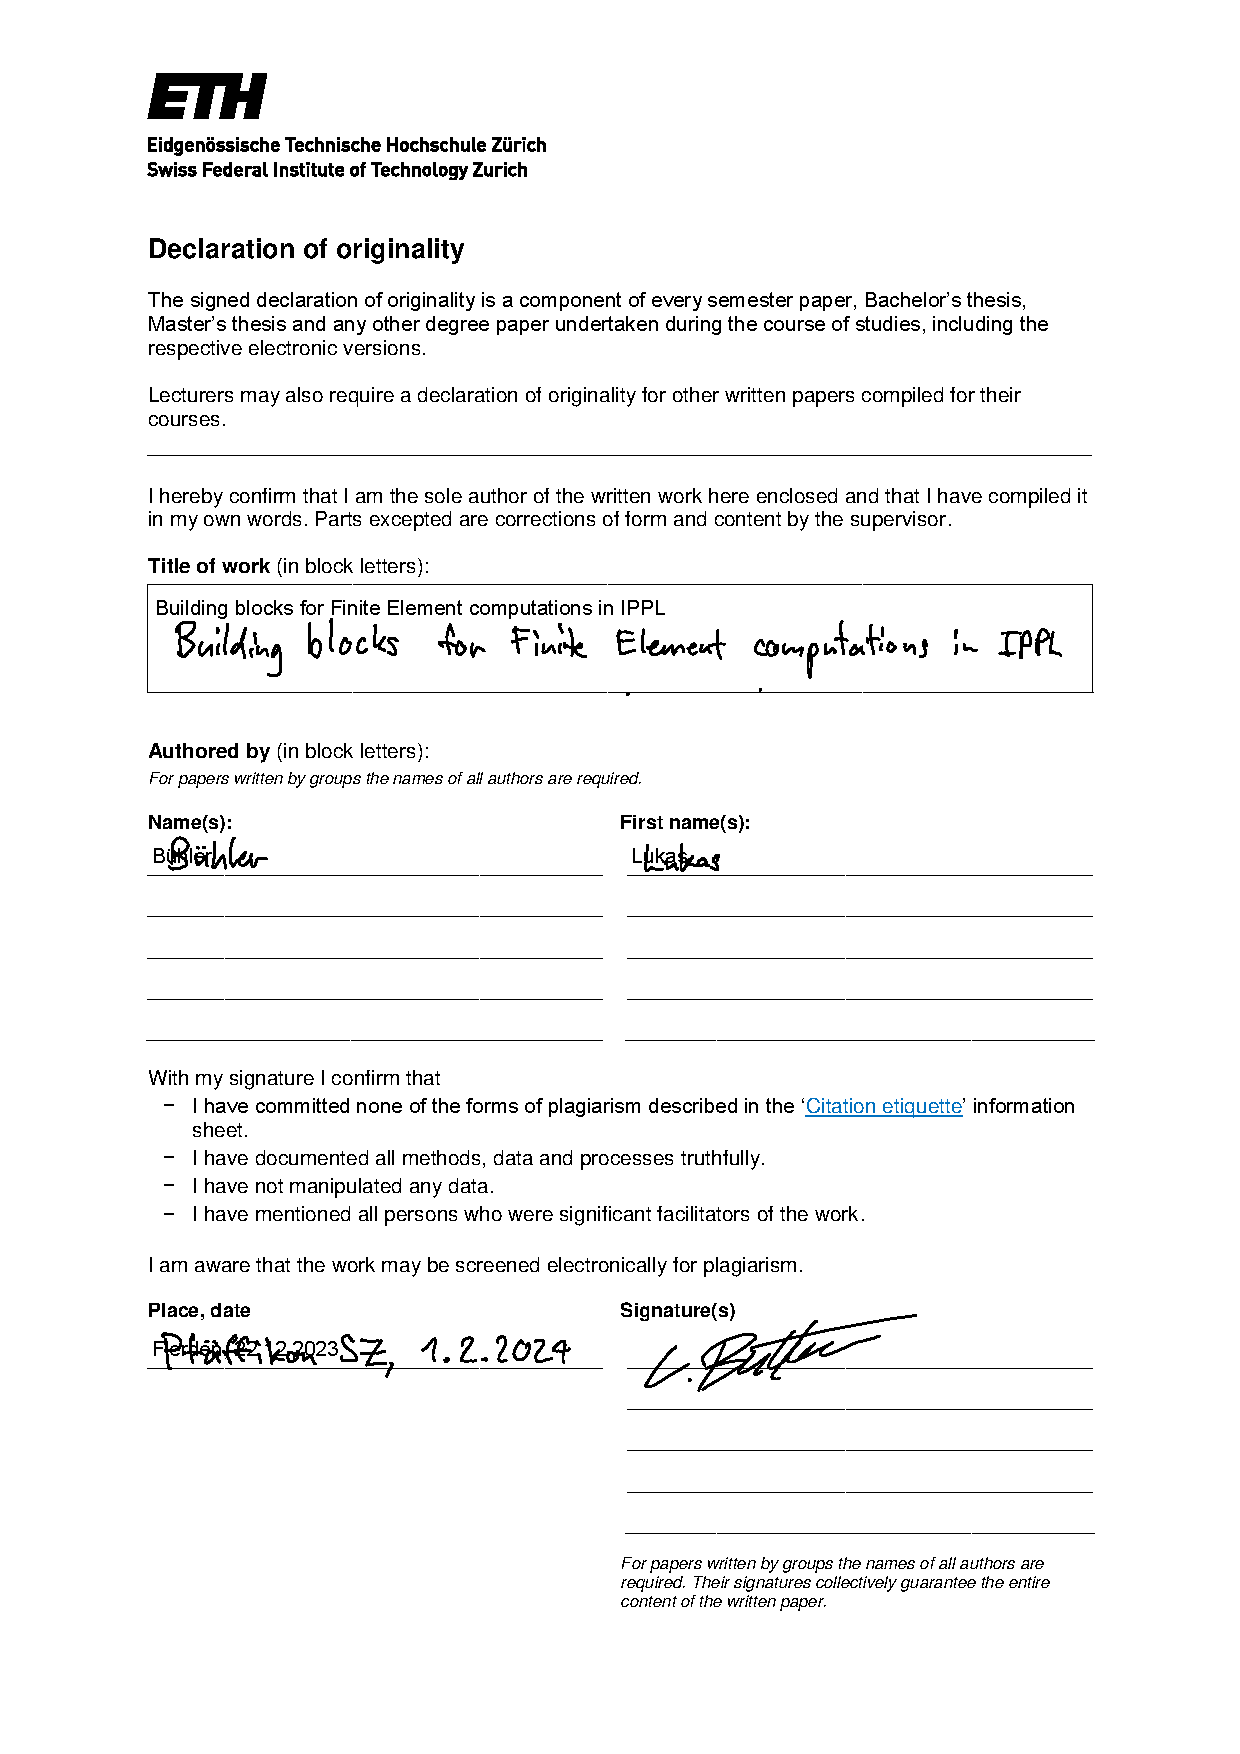
\includepdf[pages={-}]{declaration-originality-signed.pdf}

\end{document}

